\documentclass[
 reprint,
 superscriptaddress,
 nofootinbib,
 nobibnotes,
 amsmath,
 amssymb,
 aps,
 prd,
 floatfix,
 longbibliography
]{revtex4-1}

\usepackage[T1]{fontenc}
\usepackage[utf8]{inputenc}
\usepackage{amsmath,amssymb,bm}
\usepackage[draft]{graphicx}
\usepackage{booktabs}
\usepackage{dcolumn}
\usepackage[mathlines]{lineno}
\usepackage{xcolor}
\usepackage{hyperref}
\usepackage{orcidlink}

\renewcommand{\arraystretch}{1.5}

\newcommand\Jc[1]{{\color{orange}\bfseries #1}}
\newcommand\Add[1]{{\color{red}\bfseries #1}}
\newcommand\Delete[1]{{\color{cyan}\bfseries #1}}

\newcommand{\sm}{\small}
\newcommand{\Rvir}{R_{\rm vir}}
\newcommand{\rvir}{R_{\rm vir}}
\newcommand{\mvir}{M_{\rm vir}}
\newcommand{\msun}{{\rm M}_{\odot}}
\newcommand{\mstar}{{\rm M}_{*}}
\newcommand{\msunh}{h^{-1}{\rm M}_{\odot}}
\newcommand{\mhalo}{M_{\rm h}}
\newcommand*{\lsim}{\mathord{\sim}}

\hypersetup{
    pdfnewwindow=true,
    colorlinks=true,
    linkcolor=blue,
    citecolor=blue,
    filecolor=blue,
    urlcolor=blue
}

\newcommand\geant{\texttt{Geant4}}
\newcommand\gsolar{\texttt{G4SOLAR}}
\newcommand\nof{\texttt{NoField}}
\newcommand\quiet{\texttt{Quiet}}
\newcommand\act{\texttt{Active}}

\newcommand{\red}[1]{\textcolor{red}{#1}}
\newcommand{\blue}[1]{\textcolor{blue}{#1}}
\newcommand{\purple}[1]{\textcolor{purple}{#1}}

\def\apj{ApJ}
\def\aap{A\& A}
\def\apjl{ApJL}
\def\apjs{ApJS}
\def\mnras{MNRAS}
\def\jcap{JCAP}
\def\pasa{PASA}
\def\aj{AJ}
\def\araa{ARA\& A}
\def\nat{Nature}
\def\prd{Phys. Rev. D}
\def\ssr{Space Sci. Rev.}
\def\rmxaa{RMxAA}
\def\na{New Astron}
\def\jqsrt{J. Quant. Spec. Radiat. Transf.}
\def\physrep{Phys. Rep.}
\def\pasj{PASJ}

\begin{document}

\title{The Impact of Small-scale enhanced Primordial Power Spectrum on Nonlinear Structure Formation}

\author{Haina Huang\orcidlink{0009-0004-4765-0358}}
\thanks{\scriptsize \!\! Contact Author}
\email{hhuan155@link.cuhk.edu.hk}
\affiliation{Department of Physics, The Chinese University of Hong Kong, Shatin, Hong Kong, China}

\author{Tsang Keung Chan\orcidlink{0000-0003-2544-054X}}
\thanks{\scriptsize \!\! Contact Author}
\email{tsangkeungchan@cuhk.edu.hk}
\affiliation{Department of Physics, The Chinese University of Hong Kong, Shatin, Hong Kong, China}

\author{Jianhao Wu\orcidlink{0009-0000-7431-7885}}
\thanks{\scriptsize \!\! Contact Author}
\email{jianhao.wu@wisc.edu}
\email{jianhao.wu@link.cuhk.edu.hk}
\affiliation{Department of Physics, University of Wisconsin-Madison, Madison, WI, USA}
\affiliation{Department of Physics, The Chinese University of Hong Kong, Shatin, Hong Kong, China}

\date{\today}

\begin{abstract}
Using high-resolution cosmological simulations, we investigate the effects of a blue-tilted primordial power spectrum---the enhanced power on small-scale (<1Mpc)---on dark matter halos and their substructures. Initial conditions were generated from a standard power-law spectrum or two blue-tilted variants and subsequently evolved using a high-performance N-body code. We find that blue-tilted models significantly increase the abundance of low-mass ($10^9$ solar mass) halos. The amplification of the nonlinear power spectrum is stronger at high redshift and weakens at low redshift. We find halos in the blue-tilted models form earlier and have higher central densities. These results demonstrate that modifications to the primordial spectrum produce pronounced and redshift-dependent nonlinear effects, offering a theoretical basis for probing early-universe physics, for example, like strong and weak gravitational lensing observations. {\color{red}(add galaxy observation) Compared against }
\end{abstract}

\maketitle

\section{Introduction\label{intro}}
The standard cosmological model, combining single-field slow-roll inflation with the $\Lambda$ Cold Dark Matter ($\Lambda$CDM) paradigm, has achieved remarkable success in describing the large-scale structure of the Universe. Observations of the cosmic microwave background, large-scale galaxy surveys, and the Lyman-$\alpha$ forest are all in excellent agreement with predictions based on a nearly scale-invariant primordial power spectrum (PPS). However, on smaller scales (corresponding to wavenumbers $k \gtrsim 1\ \mathrm{Mpc}^{-1}$), the model faces a series of challenges, including the ``missing satellites'', ``core-cusp'', and ``too-big-to-fail'' problems \citep{Bullock17smallscalechallenges,Sales22challenges}. Recently, the James Webb Space Telescope (JWST) has detected a substantial number of massive galaxies at high redshifts ($z > 10$), whose abundance may exceed the predictions of the standard model (e.g. \cite{Hira24bluetilt}), further intensifying the theoretical tension on small scales.

In response to these challenges, various models that modify the primordial power spectrum on small scales have been proposed. Among these, the blue-tilted (BT) model emerges as a natural extension. Crucially, the model introduces a pivot scale $k_p$ (typically $\gtrsim 1\ \mathrm{Mpc}^{-1}$) that separates the well-measured large scales from the unconstrained small scales. On large scales ($k < k_p$), the spectral index retains the red-tilted value $n_s \approx 0.965$ precisely measured by Planck, ensuring full consistency with CMB observations. Only on small scales ($k > k_p$) does the spectral index become blue ($n_s > 1$), boosting the small-scale power without disturbing the observationally successful large-scale predictions. This ``decoupling'' feature allows the BT model to address small-scale tensions while remaining firmly anchored to the established cosmological framework.

Beyond high-redshift galaxies, distinguishing between different primordial power spectrum models requires other independent cosmological probes. Flux-ratio anomalies in strong gravitational lensing systems may reflect the abundance of dark matter subhalos within lens galaxies, a quantity that standard $\Lambda$CDM simulations might underproduce. Furthermore, the density profiles, abundance, and spatial distribution of nearby dwarf galaxies provide crucial information for constraining both the primordial power spectrum and the physics of galaxy formation.

Within this context, this study aims to provide, for the first time via high-resolution cosmological simulations, a systematic and quantitative investigation of the impact of a blue-tilted primordial power spectrum on the internal structure and statistics of dark matter halos.
% {\color{red} The following should be in method section} We employ \textsc{Music2-MonofonIC} to generate initial conditions based on both the standard power-law spectrum and the blue-tilted spectrum, and evolve them using the high-precision \textsc{SWIFT} $N$-body code. To ensure robust identification of halos, we utilize and compare the particle-tracking-based \textsc{HBT+} algorithm. By systematically comparing a suite of key statistics—including the halo mass function, density profiles, concentration-mass relation, half-mass formation redshift, and nonlinear matter power spectrum—between the two PPS models, we seek to uncover the distinct, multi-dimensional imprints of the blue-tilted model. Our goal is to establish a solid theoretical foundation and generate testable predictions for probing the physics of the primordial Universe with next-generation, multi-messenger observational data from facilities such as JWST, Euclid, LSST, and strong lensing surveys.(Pending modification)

\section{Theoretical Overview}
\label{sec:theory}

This study investigates the imprints of a modified primordial power spectrum (PPS) on the late-time distribution of dark matter halos and subhalos. The theoretical framework connects the physics of the early universe, set during inflation, to the nonlinear structure formation observed today, and motivates the specific models we simulate.

\subsection{From Primordial Perturbations to Cosmic Structure}
The statistical properties of the density field in the late universe are seeded by quantum fluctuations amplified during the inflationary epoch. These initial conditions are characterized by the primordial power spectrum, $P_{\mathcal{R}}(k)$. In the standard $\Lambda$CDM cosmology, a nearly scale-invariant spectrum, $P_{\mathcal{R}}(k) \propto k^{n_s}$ with $n_s \approx 0.96$, is assumed. This spectrum undergoes linear evolution described by the transfer function $T(k)$ and growth factor $D(a)$ to yield the linear matter power spectrum, $P_{\mathrm{lin}}(k, a) \propto D^2(a) T^2(k) P_{\mathcal{R}}(k)$. The subsequent gravitational collapse and nonlinear evolution of overdensities lead to the formation of a hierarchical network of dark matter halos, whose internal structure and abundance serve as fundamental probes of the underlying cosmology.

\subsection{The Blue-Tilted Power Spectrum Model}
We consider a phenomenological extension to the standard PPS, the blue-tilted (BT) model, defined by a broken power-law form:
\begin{equation}
    P_i (k) \propto \begin{cases} k^{n_s},&\left(\text{for } k<k_p\right),\\
    \frac{k}{k_p}^{m_s-n_s} k^{n_s}, &\left(\text{for } k>k_p\right),
\end{cases}
\end{equation}
where $k_p$ is a pivot wavenumber, $m_s$ is the spectral index on scales $k > k_p$, and $A_s$ and $k_0$ are the standard amplitude and pivot scale, respectively. This model preserves consistency with large-scale CMB and galaxy survey constraints ($k < k_p$), while enhancing power on smaller scales ($k > k_p$) when $m_s > n_s$ (blue-tilt). The case $m_s < n_s$ corresponds to a red-tilted (RT) model. \Jc{Do we need to mention $A_s$ here? Seems we do not directly change this param here.}

\subsection{Model Selection and Cosmological Motivation}
We focus on two specific BT models, with parameters adopted from previous BT studies on JWST early massive galaxies\cite{Hira24bluetilt} and enhancing MW substructures \citep{Wu25BT}:
\begin{itemize}
    \item \textbf{BT\_soft}: A model with a relatively low pivot scale ($k_p \approx 1.0$ Mpc$^{-1}$) and moderate enhancement ($m_s \approx 1.5$).
    \item \textbf{BT\_deep}: A model with a higher pivot scale ($k_p \approx 10$ Mpc$^{-1}$) and similar spectral tilt.
\end{itemize}
These two models allow us to explore the scale-dependence of the BT modification's effects. For comparison, we also simulate the standard power-law (PL) model ($m_s = n_s$), which serves as our baseline.

\begin{figure}[t]
    \centering
    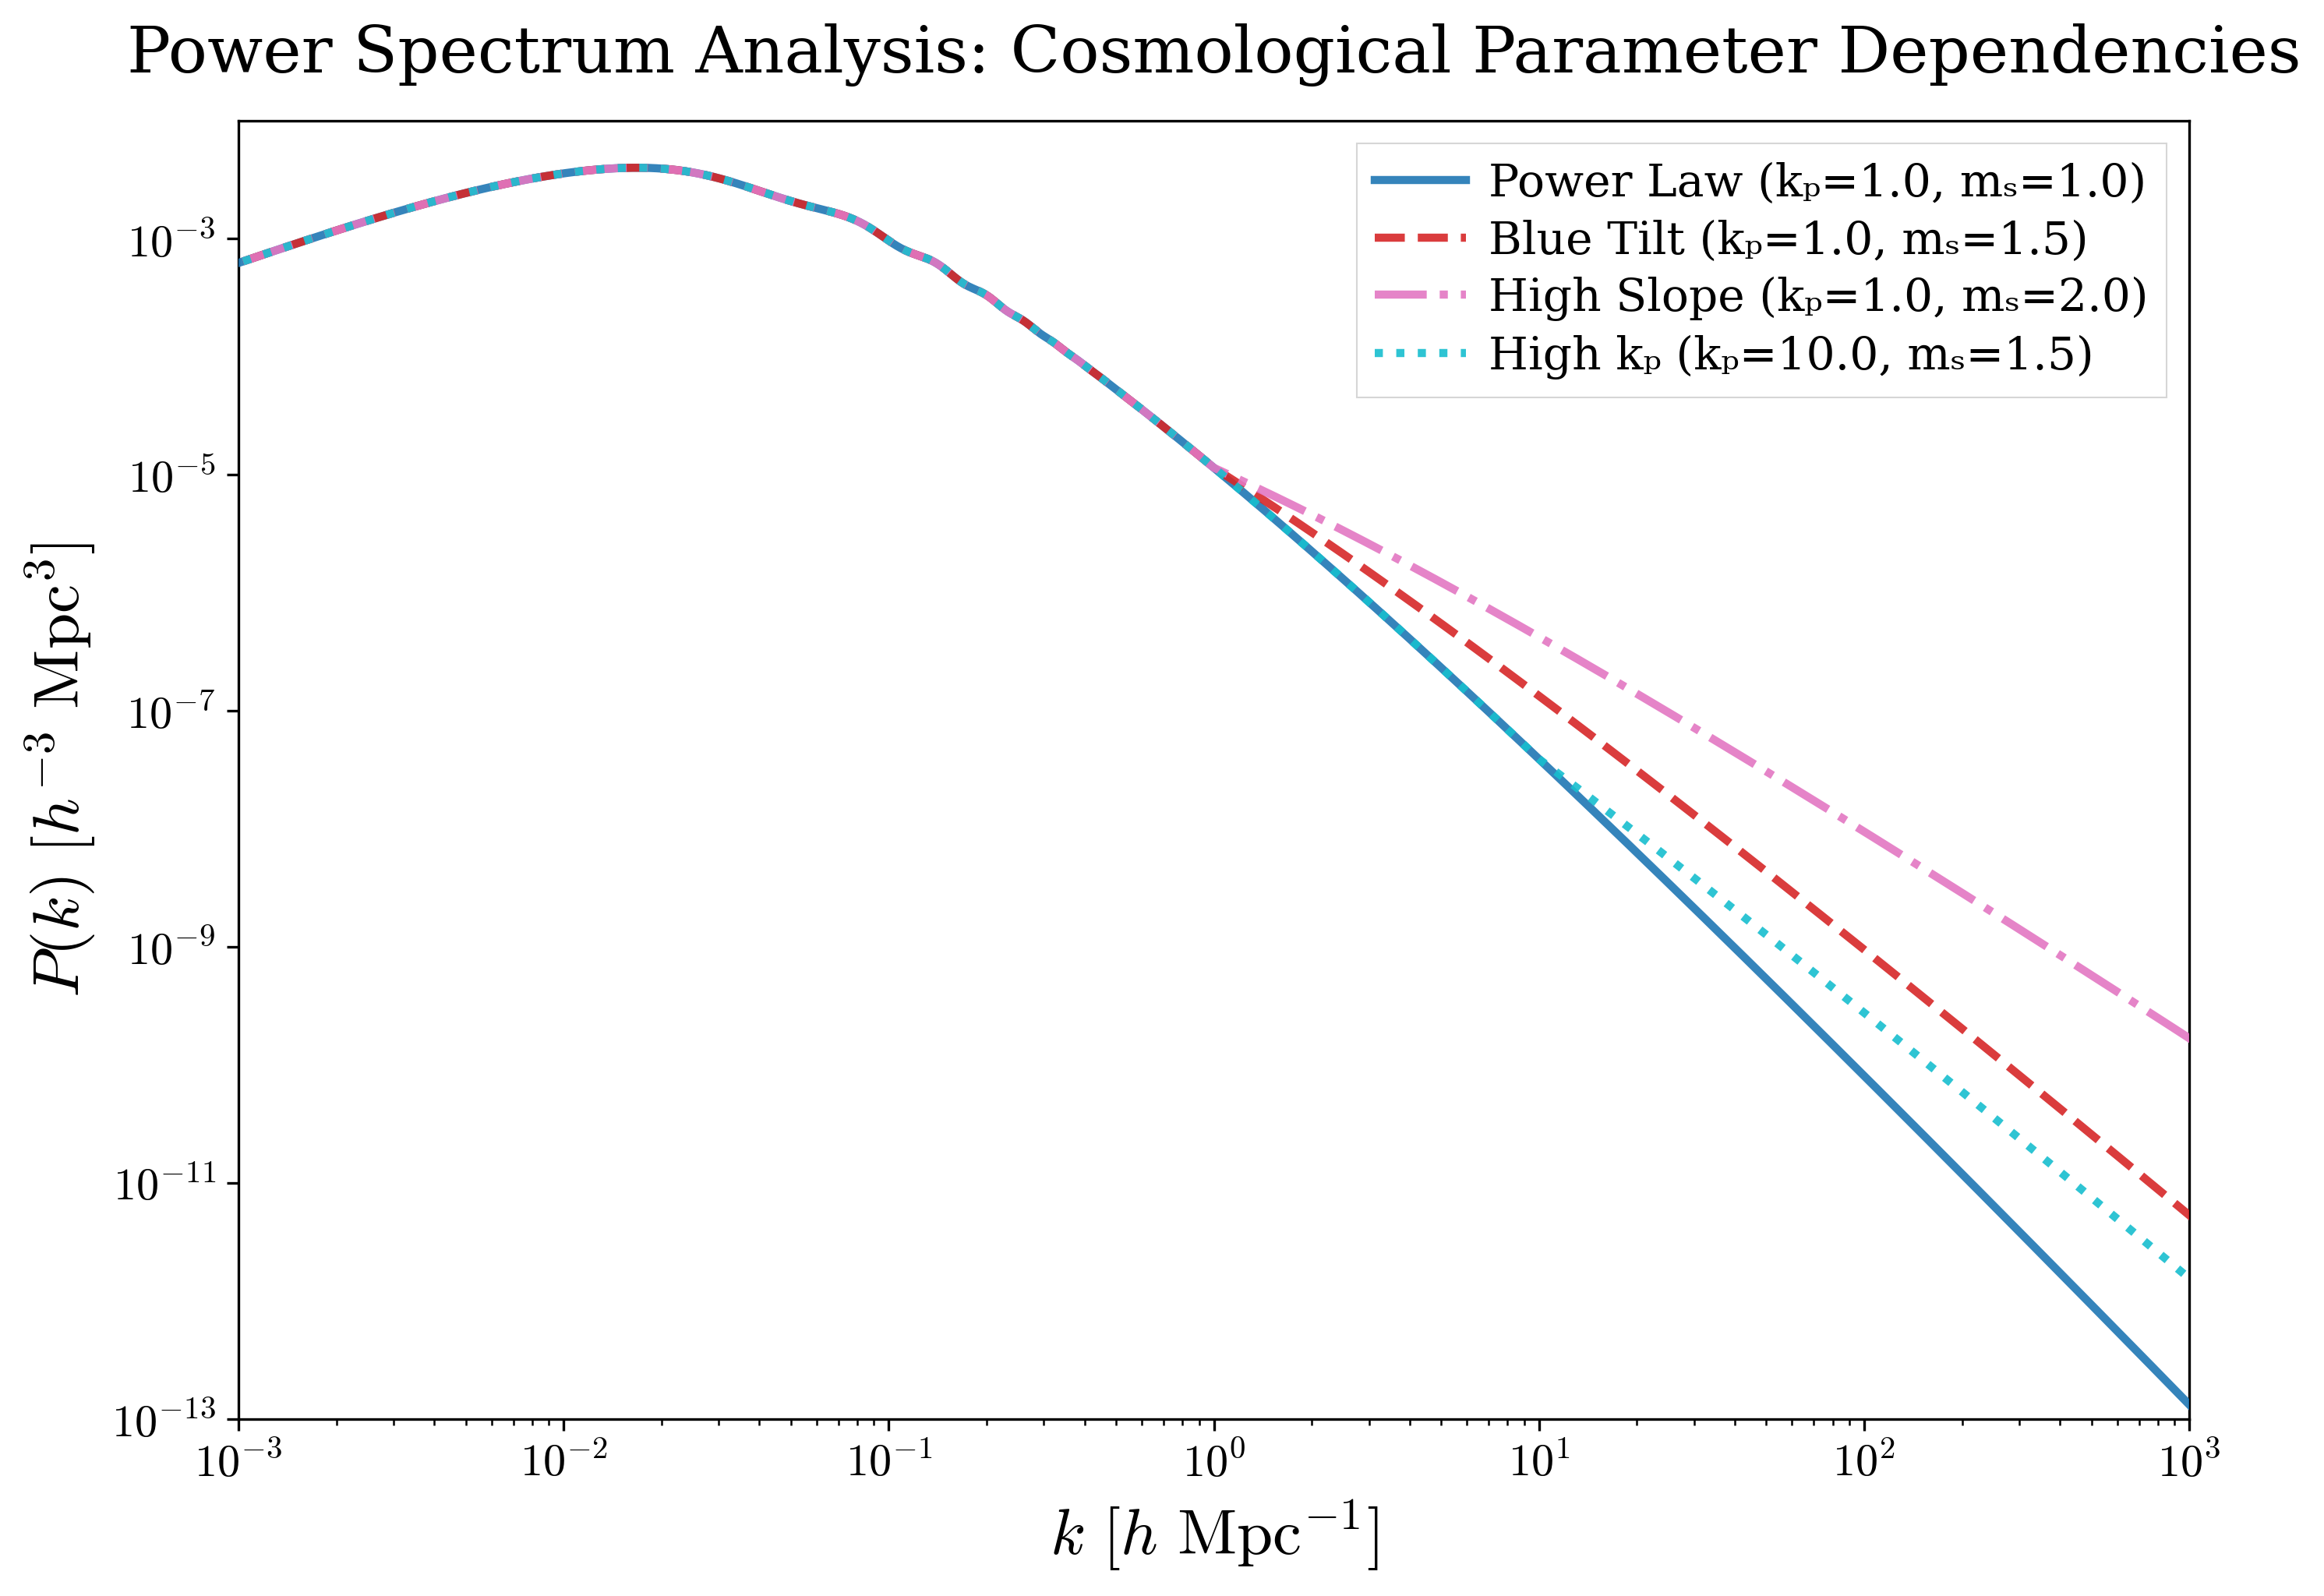
\includegraphics[scale=0.3]{power_spectrum_comparison.png}
    \caption{Matter power spectrum comparison for different spectral index parameters ($m_s$) and pivot scales ($k_p$) within the $\Lambda$CDM cosmological framework. The four curves represent: (1) Reference $\Lambda$CDM model with $m_s=0.9665$ and $k_p=0.05$ Mpc$^{-1}$ (purple solid line), (2) Modified spectral index with $m_s=1.0$ and $k_p=0.05$ Mpc$^{-1}$ (red dashed line), (3) Adjusted pivot scale with $m_s=0.9665$ and $k_p=0.02$ Mpc$^{-1}$ (blue dotted line), and (4) Combined variation with $m_s=1.0$ and $k_p=0.02$ Mpc$^{-1}$ (green dash-dotted line). The power spectrum $P(k)$ is shown across scales from $k=10^{-3}$ to $10^{1}$ Mpc$^{-1}$, demonstrating how variations in primordial power spectrum parameters affect structure formation at different scales. The dashed vertical line indicates the pivot scale $k_p=0.05$ Mpc$^{-1}$ for reference. {\color{red} redshift=200}}
    \label{fig:power_spectrum_comparison}
\end{figure}

\begin{figure}[t]
    \centering
    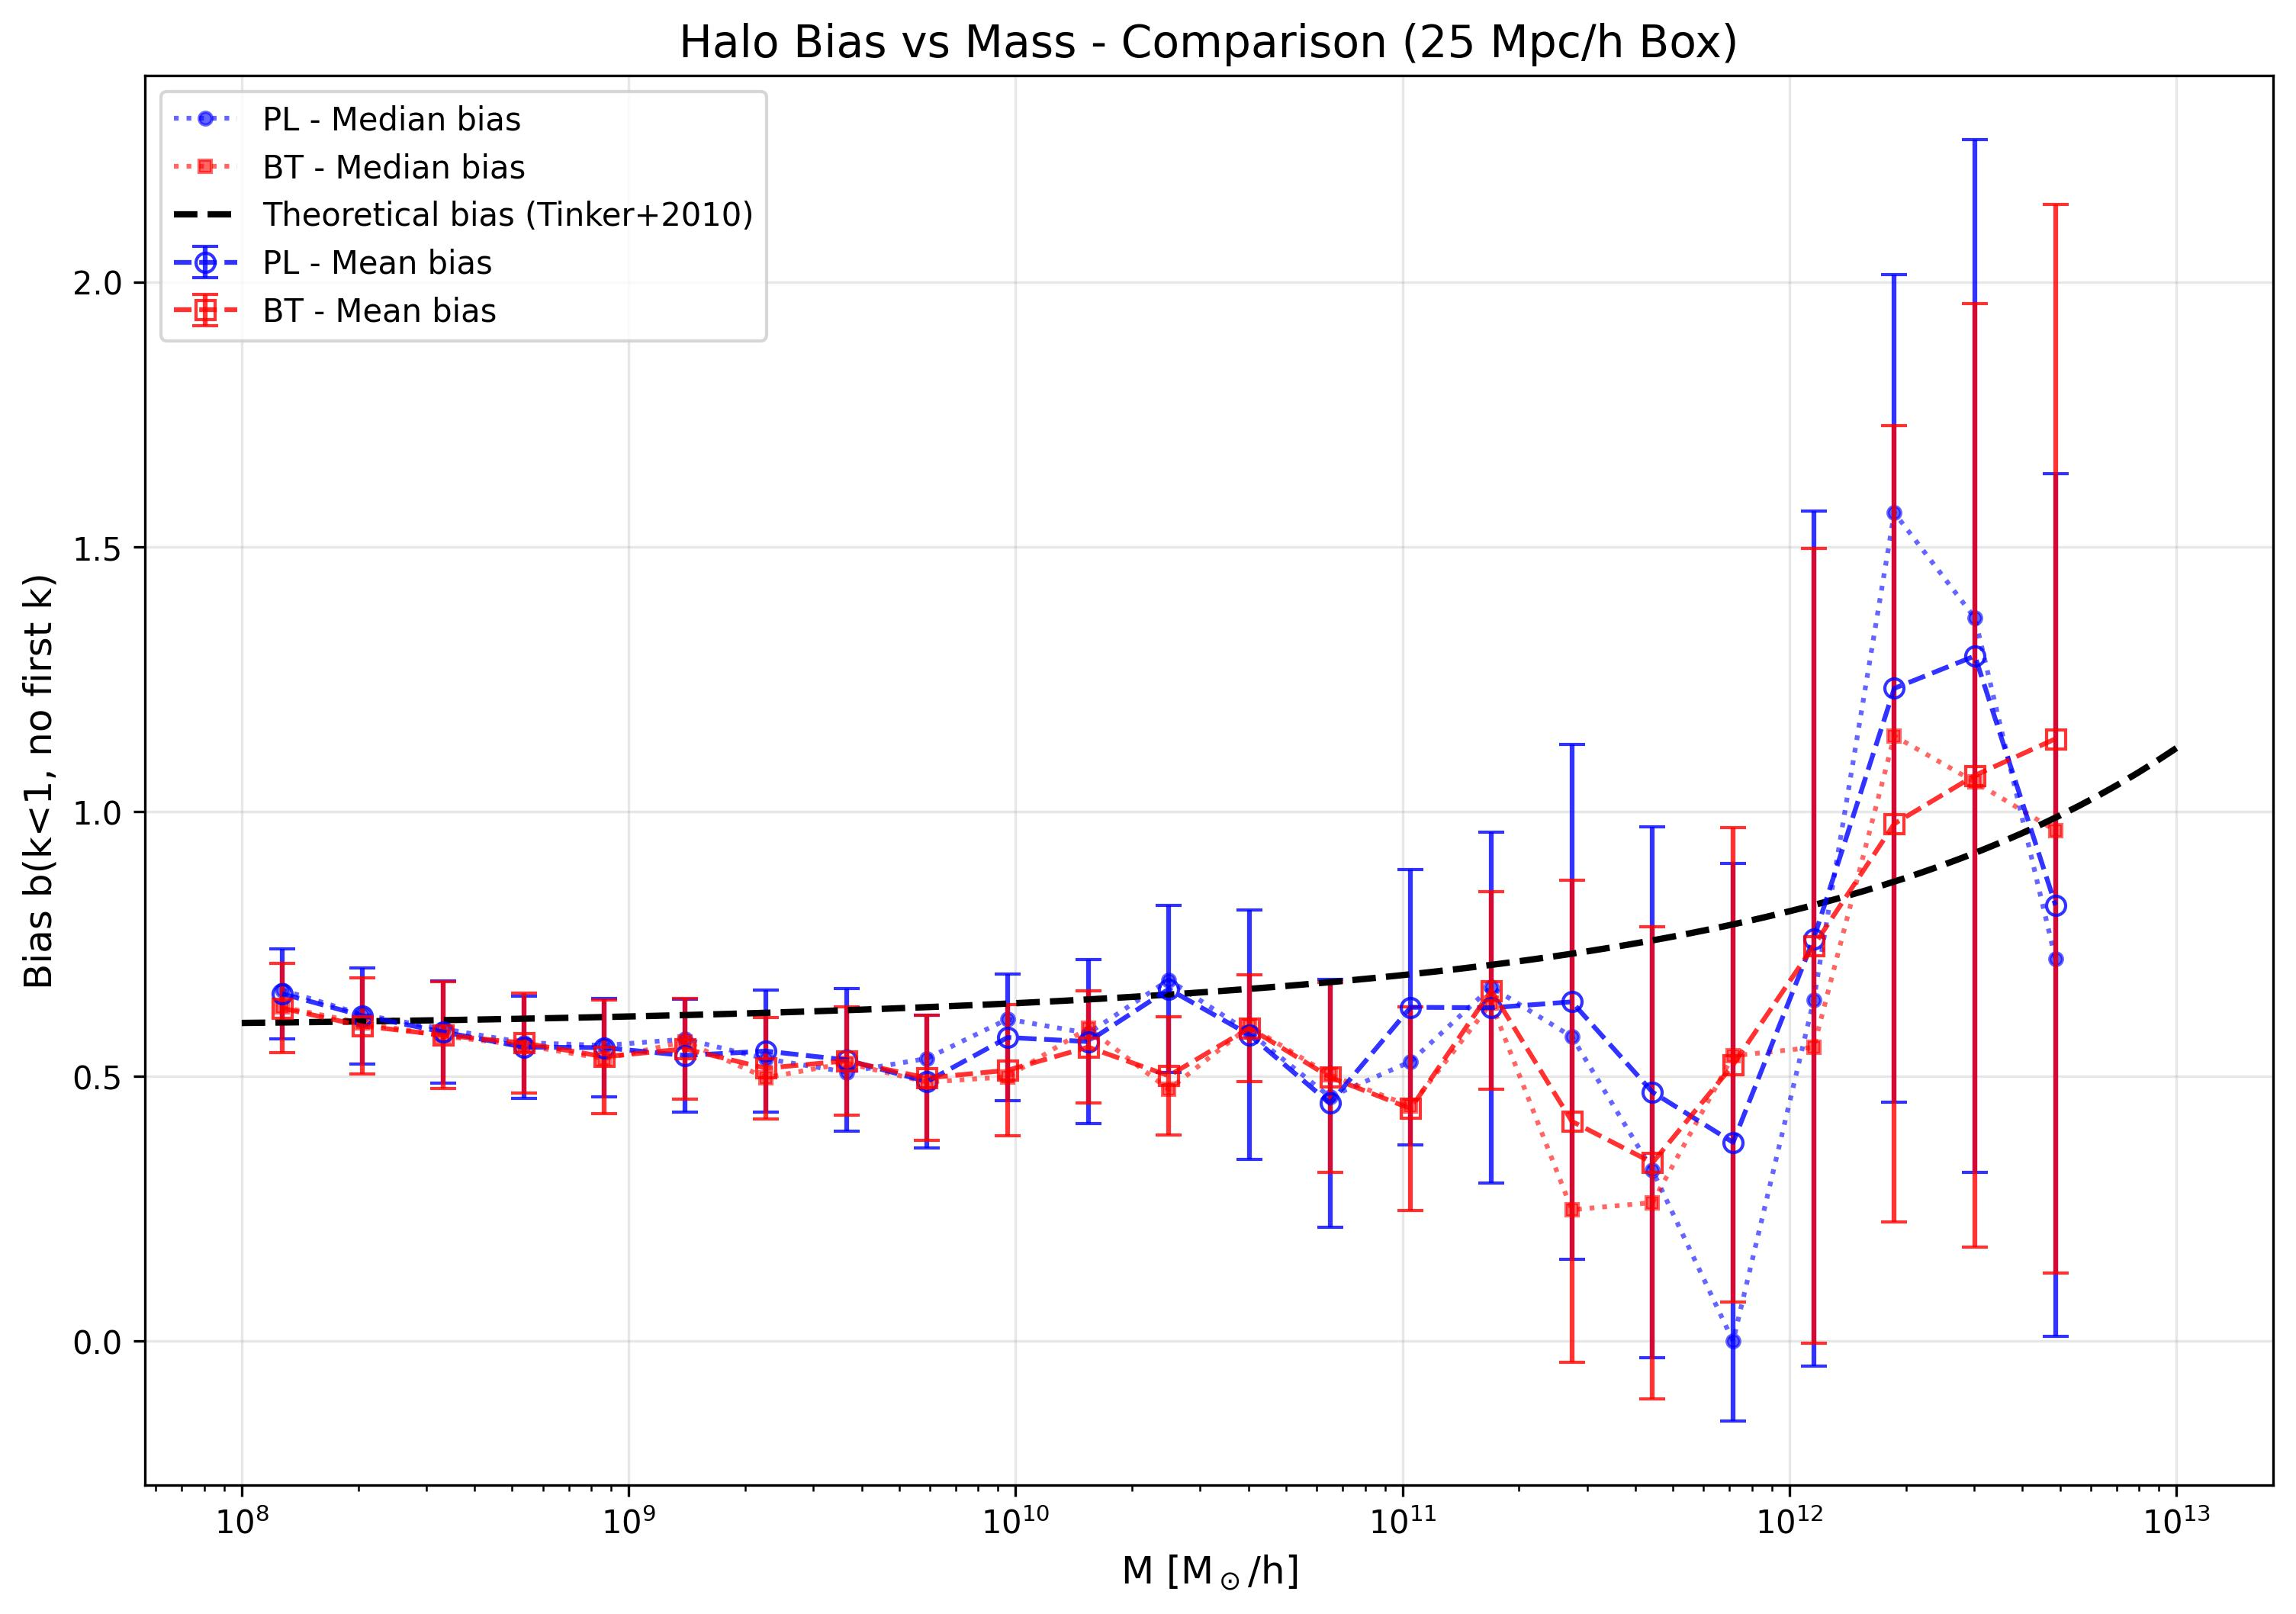
\includegraphics[scale=0.3]{bias_vs_mass_comparison_PL_vs_BT.jpg}
    \caption{Halo bias comparison across cosmological models at $z=5.0$. The figure shows the halo bias $b(M)$ as a function of halo mass for three different primordial power spectrum scenarios: standard $\Lambda$CDM (black circles), blue-tilted with $k_p=10$ (blue squares), and blue-tilted with $k_p=1$ (red triangles). All simulations use a $25$ Mpc$/h$ box with $1024^3$ particles. Error bars represent statistical uncertainties from Poisson noise in halo counts per mass bin, with a minimum threshold of 100 halos per bin. The blue-tilted models exhibit enhanced bias relative to $\Lambda$CDM, particularly at lower masses ($M \lesssim 10^8$ M$_\odot/h$), reflecting increased primordial power on small scales. The $k_p=1$ model shows stronger deviation than $k_p=10$, consistent with the broader range of scales affected by the blue tilt. This enhanced bias has important implications for early structure formation and reionization modeling in alternative cosmologies.}
    \label{fig:bias_comparison}
\end{figure}

\begin{figure}[t]
    \centering
    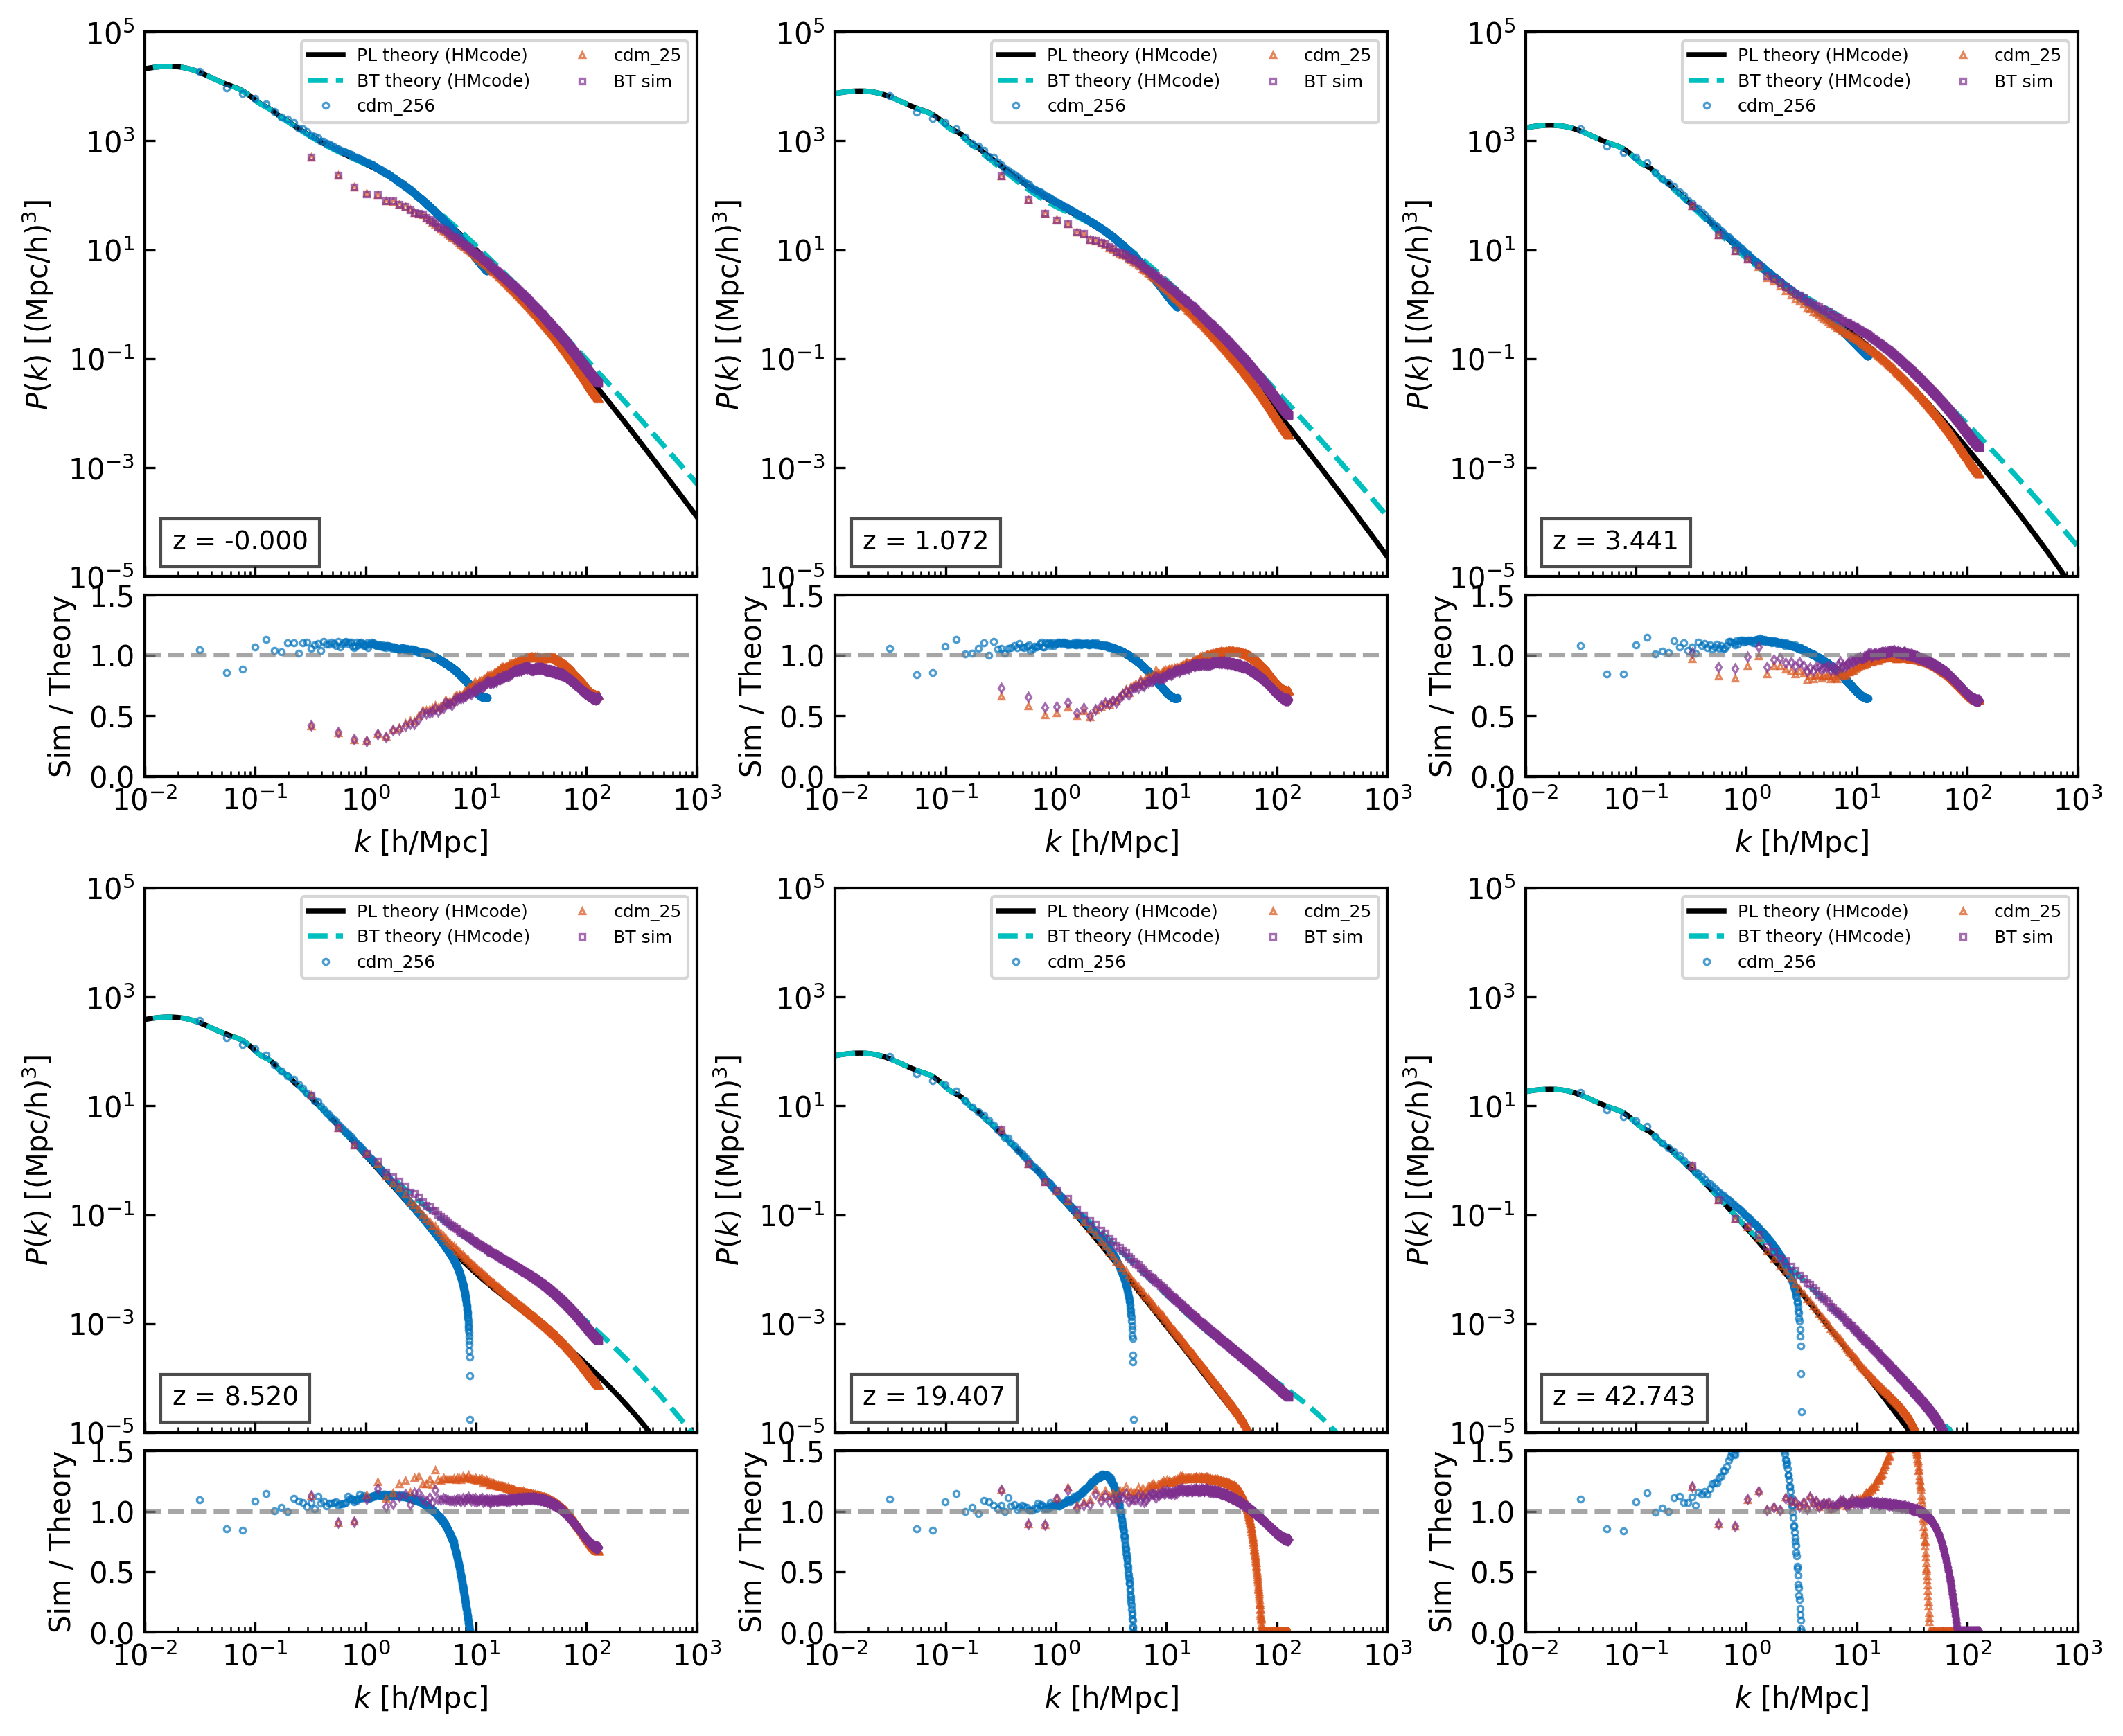
\includegraphics[scale=0.25]{HM code_vs_cdm25_cdm256_bt_with_BTtheory}
    \caption{Dark matter power spectrum comparison at redshift $z=0$. The upper panel displays the dimensionless power spectrum $\Delta^2(k)$ for three cosmological models: standard Cold Dark Matter (CDM), Blue-Tilted with characteristic scale $k_p=1$ Mpc$^{-1}$, and Blue-Tilted with $k_p=10$ Mpc$^{-1}$. These power spectra are derived from N-body simulations with $1024^3$ particles in a $25$ Mpc$^{-1}$ box. The lower panels show the ratios of Blue-Tilted models relative to CDM, revealing the suppression of small-scale power characteristic of blue-tilted initial conditions. The BT($k_p=10$ Mpc$^{-1}$) model exhibits stronger suppression at scales $k \gtrsim 1$ Mpc$^{-1}$, while BT($k_p=1$ Mpc$^{-1}$) shows milder deviations from CDM. This demonstrates how the characteristic scale $k_p$ controls the transition from standard CDM-like growth to suppressed structure formation in blue-tilted scenarios.}
    \label{fig:power_spectra_ratio_z0}
\end{figure}

\begin{table}[t]
\centering
\scalebox{1.0}{
\begin{tabular}{@{}lll@{}}
\toprule
\multicolumn{1}{l}{Models} & \multicolumn{2}{c}{Related parameters} \\
\midrule
PL & \multicolumn{2}{c}{Power Law Primordial Power Spectrum} \\
& $n_s=0.961$ \\
BT\_deep & $k_p = 3.51 \ \rm{cMpc}^{-1}$ & $m_s = 1.5$ \\
BT\_soft & $k_p = 0.702 \ \rm{cMpc}^{-1}$ & $m_s = 1.5$ \\
\bottomrule
\end{tabular}
}
\caption{The parameters of all the chosen models. $k_p$ is the wave vector at which the BT PPS would deviate from the PL PPS. $m_s$ is the enhanced spectral index for $k>k_p$, at the small scales. For other cosmological parameters, see \protect\autoref{subsub:cosmo_params}.}
\label{tab:Params_all_models}
\end{table}

\begin{figure*}[t]
    \centering
    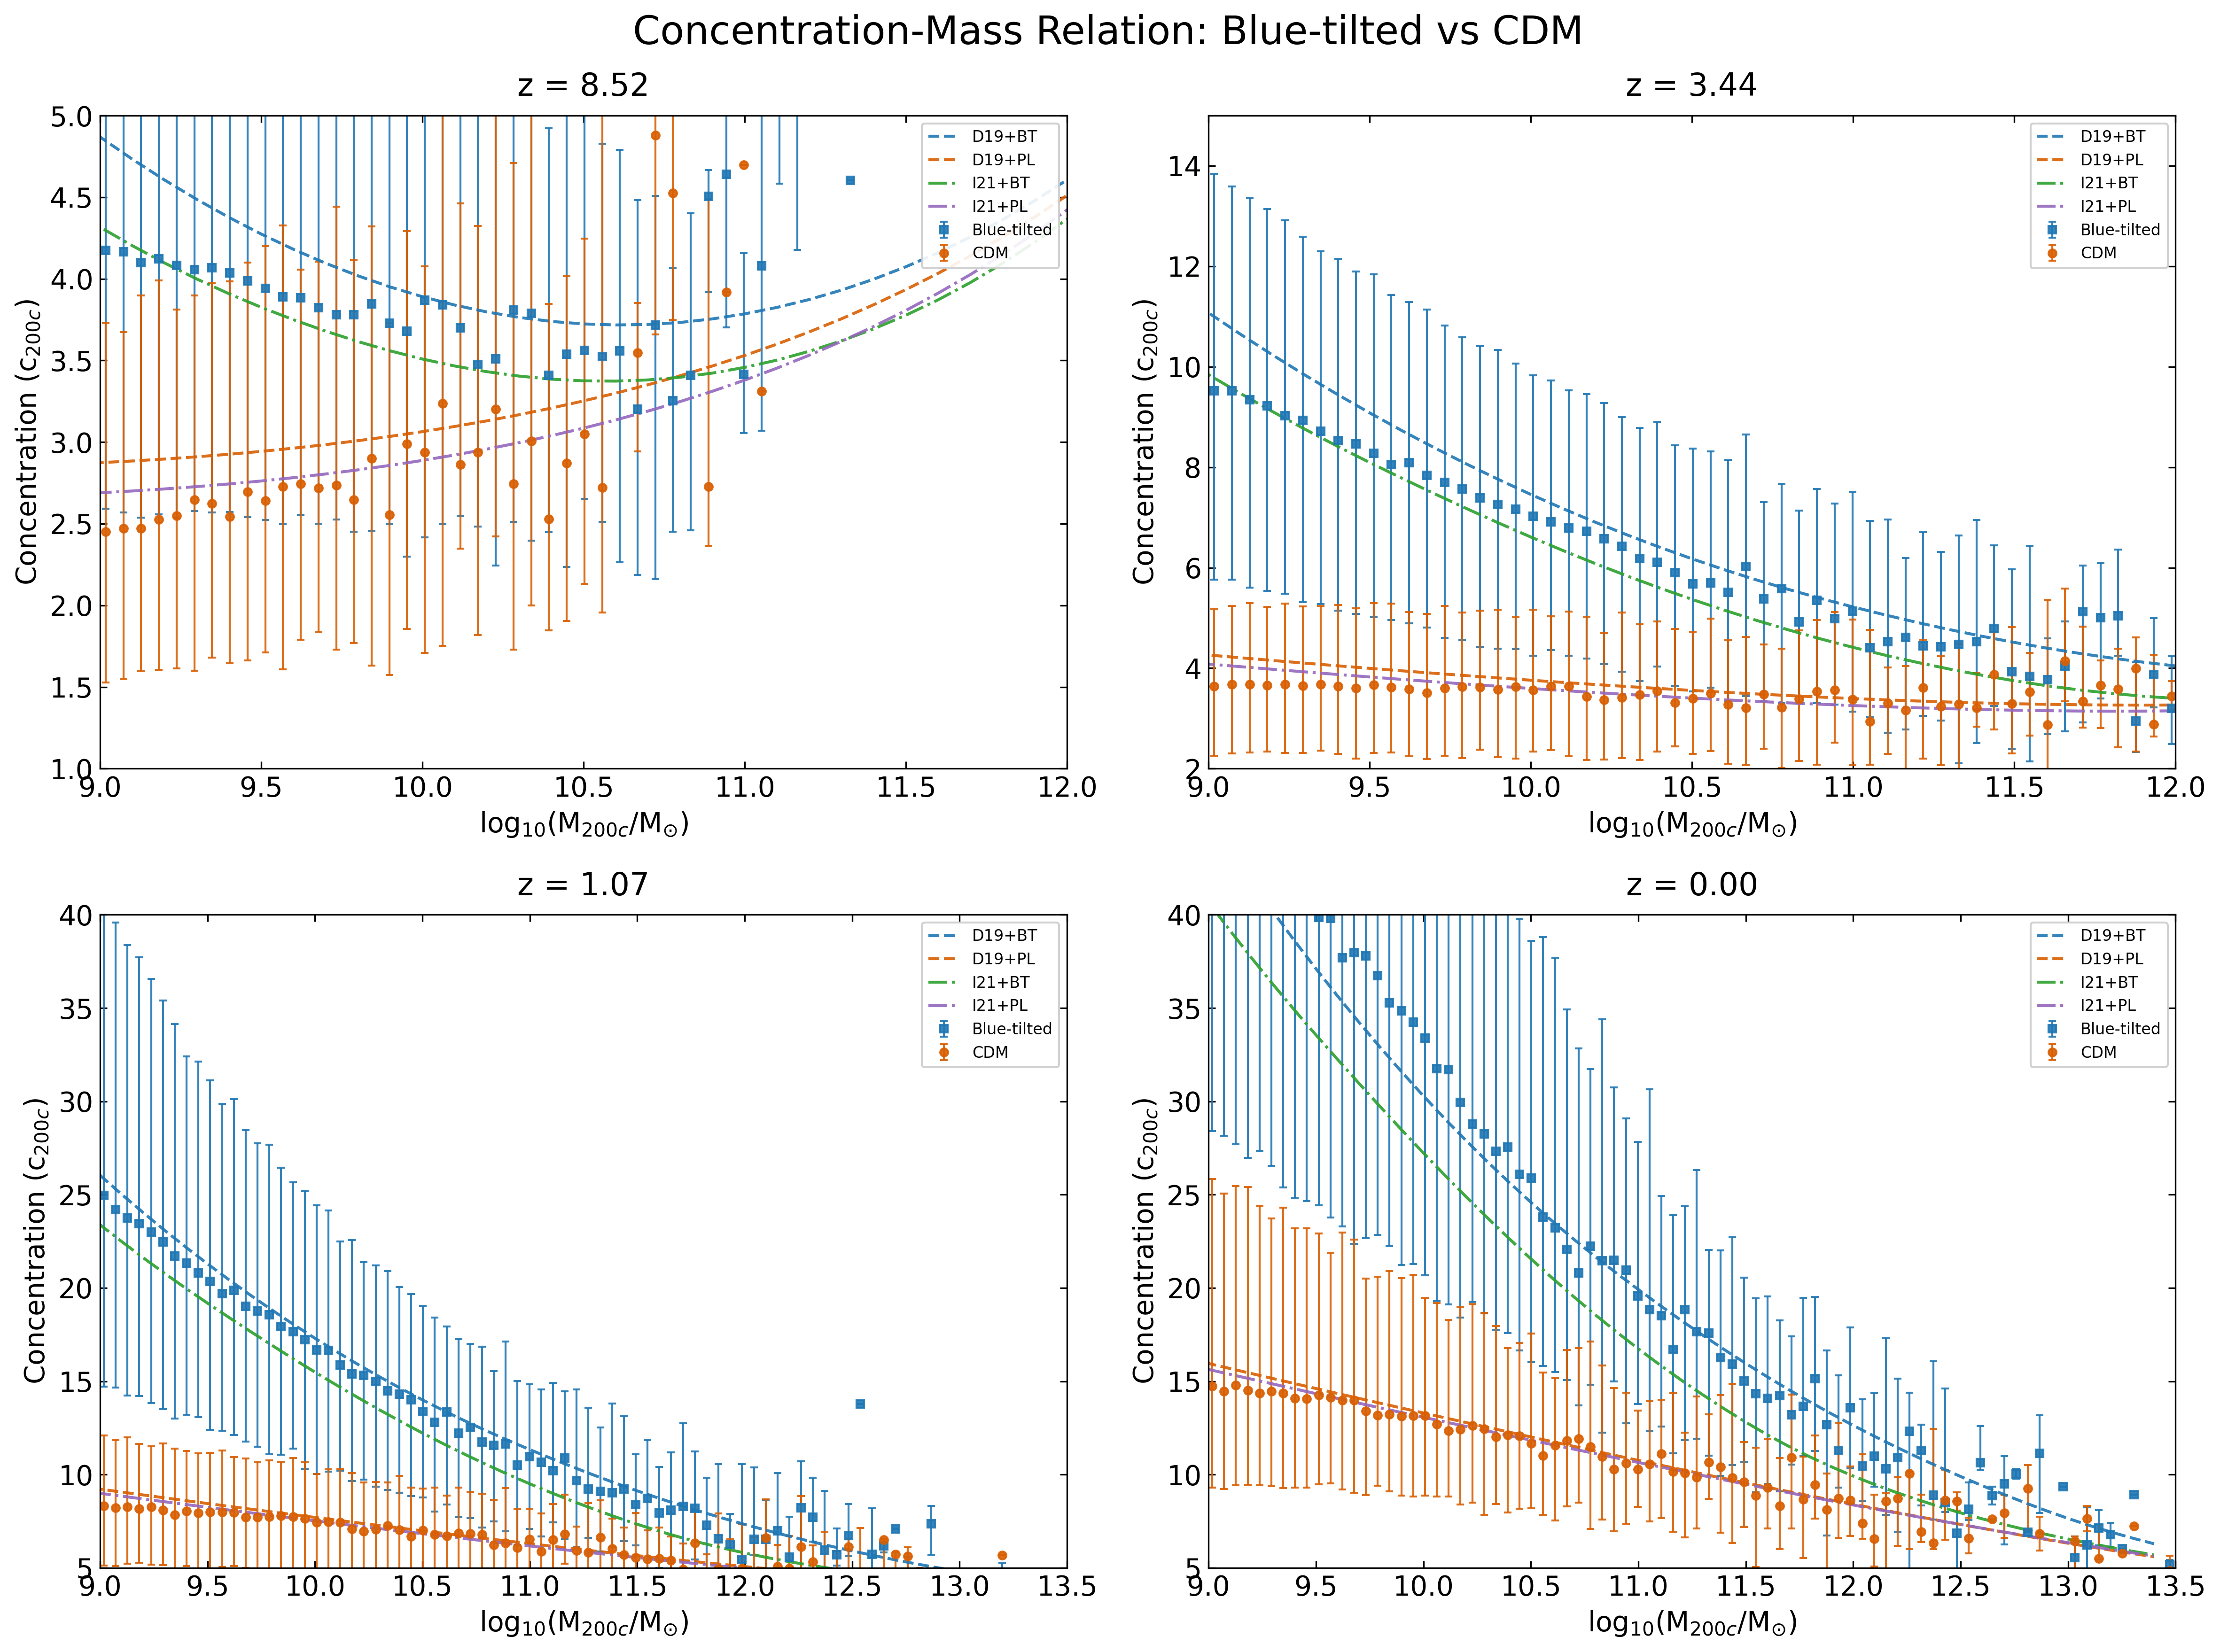
\includegraphics[scale=0.4]{concentration_four_snapshots.png}
    \caption{Dark Matter Halo Concentration-Mass Relation: Comparison of Cosmological Models 2×2 panel showing the concentration-mass relation for dark matter halos across different redshifts (z = 8.5, 3.4, 1.1, 0.0), comparing standard CDM (Cold Dark Matter) with blue-tilted power spectrum models (kp=1 and kp=10). Each panel displays three simulation datasets (circular, square, and triangular markers) with corresponding theoretical predictions (solid lines). Bottom sub-panels show the ratio of blue-tilted model concentrations relative to CDM (BT/CDM). All models use 200 times critical density mass definition and Diemer 2019 concentration model for theoretical calculations. Simulation data are from N-body simulations with 25 Mpc/h box size and 1024³ particles, with mass bins using median statistics. The plots demonstrate that blue-tilted power spectra produce higher concentration halos at high redshifts, with this effect diminishing at lower redshifts {\color{red} TK: errorbar is one-sigma scatter? can use fewer bins}.}
    \label{fig:concentration_comparison}
\end{figure*}

\begin{figure*}[t]
    \centering
    \includegraphics[scale=0.35]{dark_matter_comparison.png}
    \caption{Dark matter density field comparison between cosmological models at redshift $z=0$. The figure displays the projected dark matter density from three N-body simulations: standard Cold Dark Matter (CDM), Blue-Tilted with characteristic scale $k_p=1$ Mpc$^{-1}$, and Blue-Tilted with $k_p=10$ Mpc$^{-1}$. All simulations use $1024^3$ particles in a $25$ Mpc$^{-1}$ periodic box. The blue-tilted models exhibit reduced small-scale structure formation compared to CDM, with the suppression being more pronounced for larger $k_p$ values. This visualization demonstrates how blue-tilted initial power spectra suppress the formation of low-mass halos and filaments, leading to a smoother matter distribution at small scales while maintaining large-scale structure consistent with CDM. {\color{red} Difference is larger at higher redshift} {\color{red} The bottom right panel should be called PL instead of CDM.}}
    \label{fig:dark_matter_comparison}
\end{figure*}

\begin{figure*}[t]
    \centering
    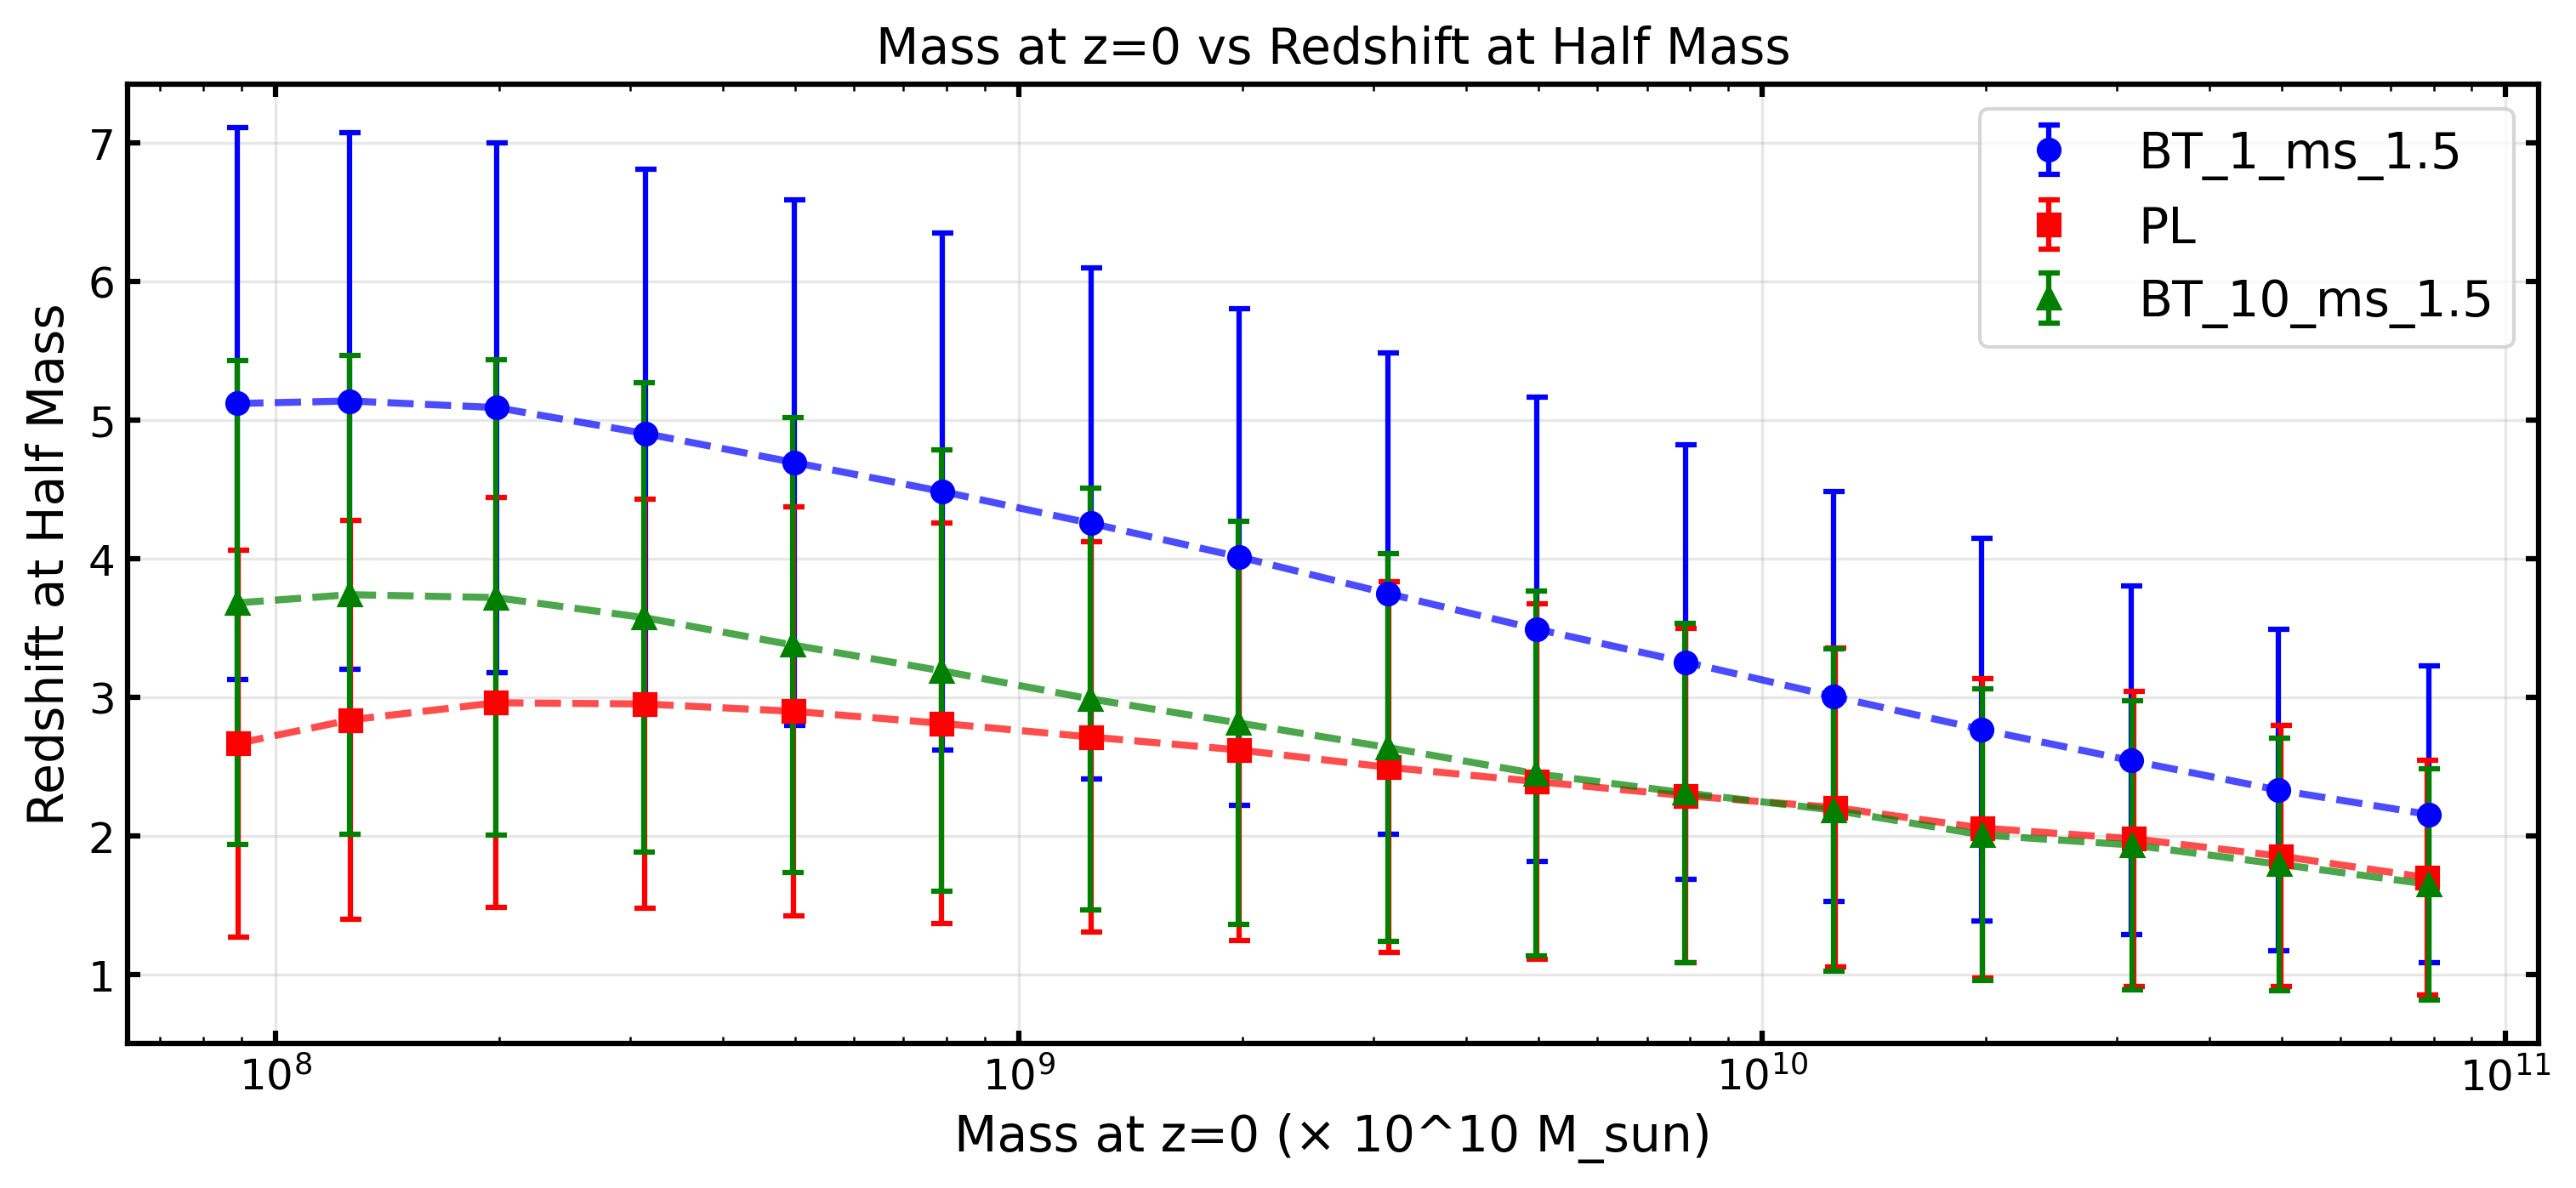
\includegraphics[scale=0.6]{mass_vs_half_mass_redshift_comparison_three_datasets.png}
    \caption{The figure compares the relationship between halo mass at redshift zero and the redshift at which halos reached half their final mass, across three different simulation datasets: BT\_1\_ms\_1.5 (blue circles), PL (red squares), and BT\_10\_ms\_1.5 (green triangles). Each data point represents the mean redshift at half mass for halos within a specific mass bin at z = 0, with error bars indicating the standard deviation of the distribution. The halo masses are multiplied by $10^{10} M_{\odot}$ for display. The dashed lines connect mass bins within each dataset, illustrating the general trend that more massive halos at z = 0 typically reached half their mass at earlier times (higher redshifts). {\color{red} TK: add COCO line or MS-II Figure 8 in \protect\cite{Hellwing16cocoproject}}}
    \label{fig:half_mass_redshift}
\end{figure*}

\section{Numerical Methods}
\label{sec:numerical}

\subsection{initial conditions (IC)}
We select the public code Music2-MonofonIC (Multi-Scale Initial Conditions for Cosmological Simulations []) to generate the initial conditions for our cosmological zoom-in simulations. We adopt the Eisenstein and Hu [] transfer function, modifying it according to the method described in Section II to simulate the blue-tilted primordial power spectrum.(Pending modification)

\subsection{Simulation code}
We perform several simulations using the state-of-the-art cosmological simulation code SWIFT []. For N-body simulations, SWIFT uses the Fast Multipole Method (FMM) at small scales [68], which can reduce the complexity of gravity calculation (including both the potential and force calculation) to O(N ). The Particle Mesh Method is also coupled at large scales to handle periodic volumes [].(Pending modification)

\subsubsection{Cosmological parameters}
\label{subsub:cosmo_params}

For all the cosmological simulations in this paper,
\begin{enumerate}
    \item Universe density parameters $\Omega_m=0.3153$, $\Omega_b=0.0493$, $\Omega_L= 0.6847$.
    \item Hubble constant $H_0 = 67.36 \ \rm{km}\ \rm{s}^{-1}\ \rm{cMpc}^{-1}$
    \item Scalar spectral index $n_s = 0.9649$
    \item Root-mean-square matter fluctuation averaged over a sphere of radius $8 h^{-1}~\rm{cMpc}$, $\sigma_8 = 0.8111$.
\end{enumerate}

\begin{table*}[t]
\centering
\small
\setlength{\tabcolsep}{4pt}
\renewcommand{\arraystretch}{1.25}
\begin{tabular}{l c c c c c c}
\hline
\hline
Model & $k_p$ & $m_s$ & $N$ & Box size & $m_{\text{DM}}$ & $\epsilon$ \\
 & $[h\,\text{Mpc}^{-1}]$ & & & $[h^{-1}\,\text{Mpc}]$ & $[h^{-1}M_\odot]$ & $[h^{-1}\,\text{Mpc}]$ \\
\hline
\textbf{Production Runs (N=1024)} \\
\hline
pl\_25\_1024   & -- & -- & $1024^3$ & 25 & $8.1\times 10^7$ & 0.000145 \\
kp\_1\_ms\_1.5\_25\_1024  & 1  & 1.5 & $1024^3$ & 25 & $8.1\times 10^7$ & 0.000145 \\
kp\_1\_ms\_2.0\_25\_1024  & 1  & 2.0 & $1024^3$ & 25 & $8.1\times 10^7$ & 0.000145 \\
kp\_10\_ms\_1.5\_25\_1024 & 10 & 1.5 & $1024^3$ & 25 & $8.1\times 10^7$ & 0.000145 \\
kp\_10\_ms\_2.0\_25\_1024 & 10 & 2.0 & $1024^3$ & 25 & $8.1\times 10^7$ & 0.000145 \\
kp\_1\_ms\_1.5\_5\_1024   & 1  & 1.5 & $1024^3$ & 5 & $1.3\times 10^6$ & 0.000029 \\
kp\_1\_ms\_1.5\_2.5\_1024 & 1  & 1.5 & $1024^3$ & 2.5 & $1.6\times 10^5$ & 0.0000145 \\
\hline
\textbf{Convergence Test Runs} \\
\hline
pl\_25\_512    & -- & -- & $512^3$  & 25 & $6.5\times 10^8$ & 0.00029 \\
pl\_25\_256    & -- & -- & $256^3$  & 25 & $5.2\times 10^9$ & 0.00058 \\
pl\_50\_512    & -- & -- & $512^3$  & 50 & $5.2\times 10^9$ & 0.00058 \\
pl\_256\_1024  & -- & -- & $1024^3$ & 256 & $1.4\times 10^{10}$ & 0.00148 \\
pl\_256\_512   & -- & -- & $512^3$  & 256 & $1.1\times 10^{11}$ & 0.00296 \\
\hline
\end{tabular}
\caption{Summary of cosmological N-body simulation parameters. PL models use standard power-law power spectra, while Blue Tilted models have enhanced power on small scales. $k_p$ is the wavenumber where the power spectrum enhancement begins, $m_s$ is the spectral index (tilt slope), $N$ is the number of dark matter particles, Box size is the comoving side length of the simulation volume, $m_{\text{DM}}$ is the dark matter particle mass, and $\epsilon$ is the gravitational softening length. All simulations use the same background cosmology with varying initial conditions to study the effects of small-scale power on structure formation.}
\label{tab:simulation_parameters}
\end{table*}

\subsection{Halo finder and halo property post-processor}
In the main text of the paper, we adopt HBT+[] (Forouhar Moreno et al in preparation) 5 as our halo finder, which is a tracking finder. In this paper, we adopt 20 as the minimum number of particles to be identified as a dark matter halo for both halo finders. We choose the position of the most bound particle as the halo center. We use SOAP (Spherical Overdensity and Aperture Processor) to calculate the spherical overdensity properties, based on the results from HBT+.(Pending modification)

\subsection{Terminology\label{subsec:Terminology}}
We run nine simulations using the numerical pipeline mentioned in section III. Their numerical settings are listed in Table II. The six fiducial-resolution simulations are used to compare the BT and the PL models. (Pending modification)

\subsection{Comparison between the PL and the BT models}\label{subsec:comparison_PL_BT}

Figure X presents the projected dark matter distribution maps from the simulations of the PL, BT\_deep, and BT\_soft models. In these three cases, the main halos appear similar in the projection maps. However, the BT model contains a significantly larger number of subhalos than the PL model, including both small and massive subhalos. In terms of spatial distribution, the substructures in the BT model are also more centrally concentrated compared to those in the PL model. In the remainder of this section, we will quantify these differences in terms of the halo mass function, Dark Matter Halo Concentration-Mass Relation, dark matter power spectrum, halo bias, dark matter halo properties, the half-mass epoch-redshift relation, the concentration-mass relation, and the halo density profile.

\subsubsection{Halo Density Profile\label{subsub:DensityProfile}}
\begin{figure*}[t]
    \centering
    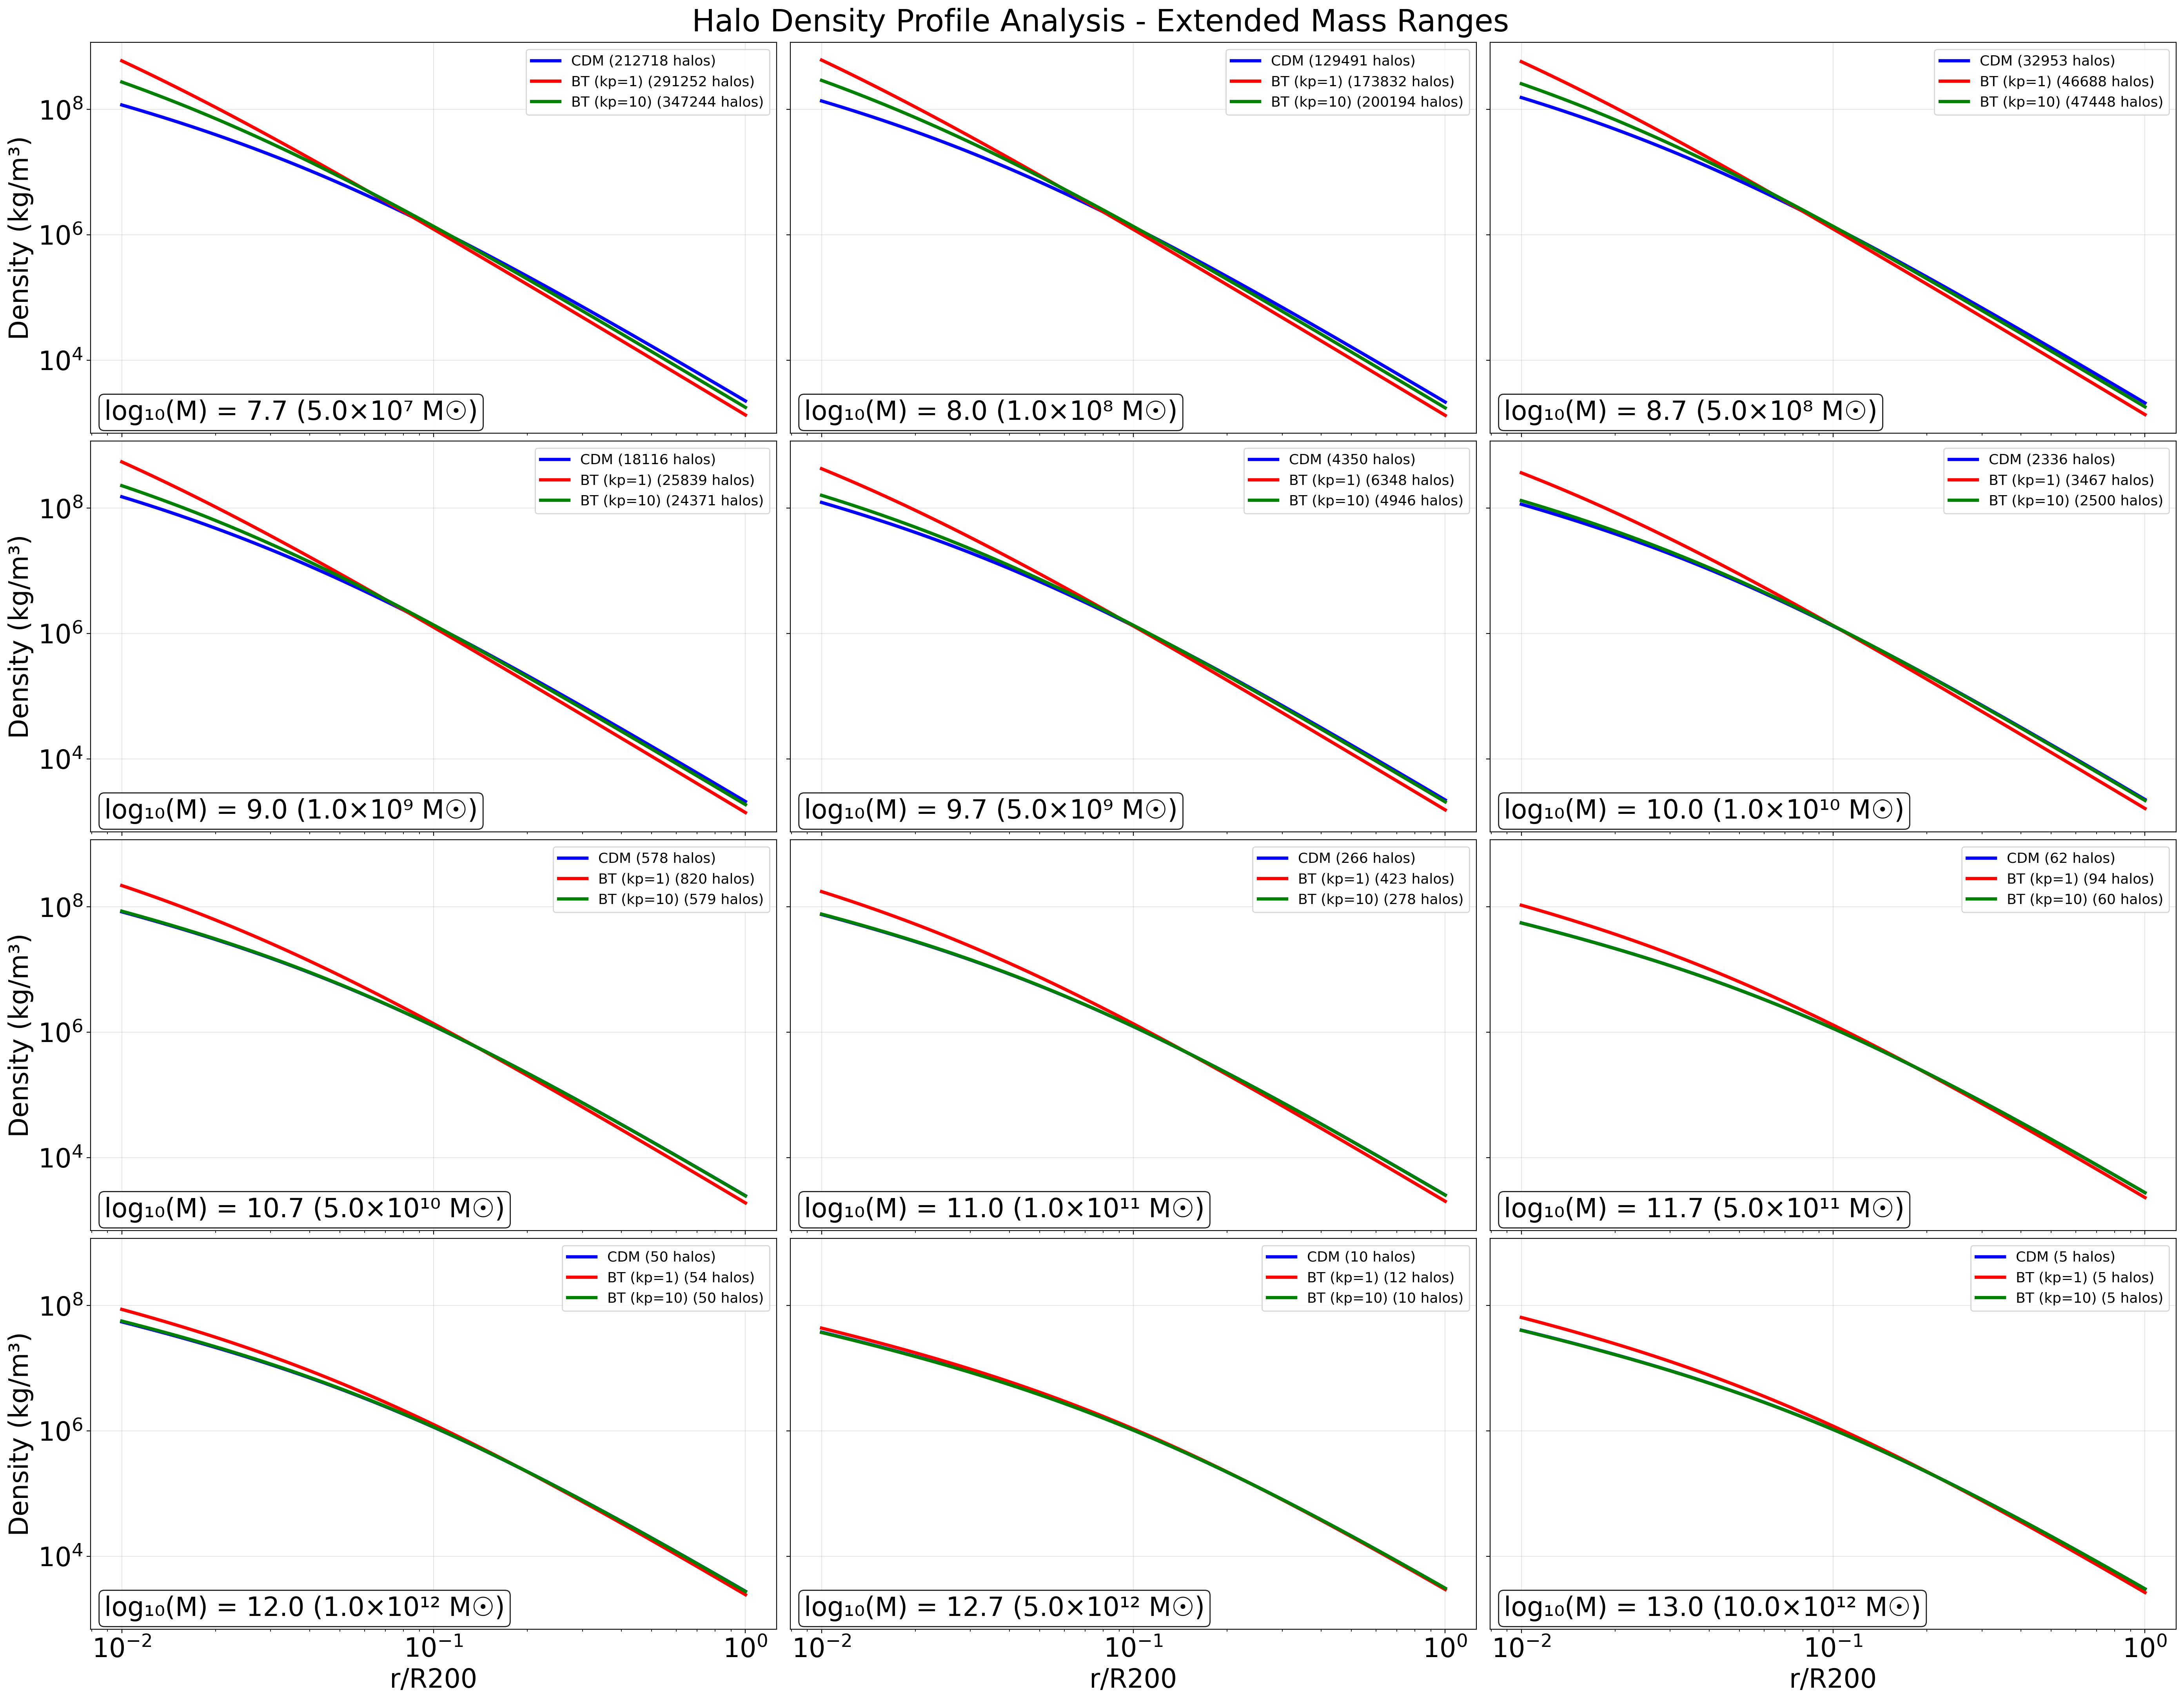
\includegraphics[scale=0.25]{halo_density_analysis.png}
    \caption{This figure presents a comprehensive comparison of halo density profiles across three cosmological models: CDM (Cold Dark Matter, blue lines), BT with kp=1 (Bluetilted model with kp=1, red lines), and BT with kp=10 (Bluetilted model with kp=10, green lines). The analysis covers 12 mass bins ranging from $5\times10^7$ M$_\odot$ to $1\times10^{13}$ M$_\odot$ ($\log_{10}(M) = 7.7$ to $13.0$), displayed in a $4\times3$ subplot grid. Each subplot shows the normalized radial density profiles ($\rho(r)$ vs. $r/R_{200}$) for halos within $\pm20\%$ of the target mass. The NFW (Navarro-Frenk-White) density profile is calculated using concentration parameters ($C_{200}$) and virial radii ($R_{200}$) derived from SOAP halo catalogs. The x-axis represents the fractional radius normalized to $R_{200}$, while the y-axis shows the density in physical units (kg/m$^3$). {\color{red} In general, we should be more clear about the kp and ms in the plot. What is the kp and ms here?}}
    \label{fig:halo_density_analysis}
\end{figure*}
Based on the analysis of our simulation data (Fig.~X), we systematically compare the density profiles of dark matter halos across the standard Cold Dark Matter (CDM) model, the strongly blue-tilted model ($k_p=1$), and the weakly blue-tilted model ($k_p=10$). The results indicate that the internal structure of halos is highly sensitive to the blue-tilted modification of the primordial power spectrum, and its response exhibits a significant radial dichotomy and mass dependence.

In the inner regions ($r < 0.1, R_{200}$), the strongly blue-tilted model ($k_p=1$) shows the most pronounced density enhancement across almost the entire mass range, followed by the weakly blue-tilted model ($k_p=10$), while the CDM model predicts the lowest central density. This suggests that the extra power on small scales in the blue-tilted power spectrum efficiently promotes the early collapse and mass concentration in the halo cores.

In the outer regions ($r > 0.3, R_{200}$), the differences between models display a clear evolution with mass. For high-mass halos ($M_h \gtrsim 10^{12} M_\odot$), the density profiles of all three models converge and are nearly indistinguishable. Moving into the intermediate mass range ($10^9 \lesssim M_h \lesssim 10^{11} M_\odot$), the outer density of the strongly blue-tilted model begins to fall systematically below that of the CDM and weakly blue-tilted models, with this density deficit increasing progressively as the halo mass decreases. At the low-mass end ($M_h \lesssim 10^8 M_\odot$), the behavior of the three models becomes distinctly stratified: the strongly blue-tilted model exhibits the most extreme signature of high inner density coupled with low outer density; the weakly blue-tilted model shows intermediate densities at all radii; whereas the CDM model is characterized by the lowest inner density but the relatively highest outer density.
This unique radial anti-correlation---inner enhancement paired with outer suppression---reveals that the blue-tilted modification not only directly affects the early formation and central collapse of halos by enhancing small-scale power but also modulates their subsequent mass accretion history in a complex, mass-dependent manner. The systematic reduction of outer density in intermediate and low-mass halos may be linked to the increased subhalo abundance, and differences in the large-scale matter distribution in blue-tilted models, the specific mechanisms of which warrant further investigation. These findings provide a novel theoretical perspective for using the global density structure of halos to precisely discriminate between and constrain different models of the primordial power spectrum.

\subsubsection{halo Mass Function\label{subsub:HMF}}

We utilize a set of high-resolution cosmological simulations to investigate the evolution of the halo mass function from high redshift (approximately $z \approx 8.5$) to the present day, aiming to place constraints on models featuring a blue-tilted primordial power spectrum. The analysis is based on three representative cosmological simulation models: the PL model employing a standard power-law power spectrum serves as the baseline, while two blue-tilted power spectrum models with differing tilt strengths (BT\_hard and BT\_soft) are used for comparative study. To trace the history of structure formation, we sampled at nine distinct epochs from high to low redshift (corresponding to snapshot numbers 32 to 56).

Halo masses are defined using the \textbf{Friends-of-Friends (FOF)} algorithm, which links dark matter particles into halos via a given linking length (typically 0.2 times the mean particle separation). These FOF halo masses are extracted from the post-processing catalogs generated by the \textsc{SWIFT} simulation. The halo mass function is calculated using the integration-averaging method {\color{red} (need to be clearer or add reference)}, which is more precise than simple histogram binning. We partition the mass range in logarithmic space with a density of six bins per mass decade. Within each bin, we compute the integral of the halo count and the mass-weighted average mass. The mass function $\frac{dn}{d\log M}$ is calculated via:
\begin{equation}
\frac{dn}{d\log M} = \frac{\int dn}{V \cdot \Delta \log M}.
\end{equation}
Statistical errors are estimated based on Poisson statistics, given by $\sigma = \sqrt{N}/(V \cdot \Delta \log M)$, where $N$ is the number of halos in the bin. The volume of the periodic simulation box is $(25\ \mathrm{Mpc}/h)^3$. To mitigate the systematic overestimation of halo masses at low particle counts, we apply the \protect\cite{Warren_2006}correction $N_{\text{corrected}} = N(1-N^{-0.6})$ to each halo's particle count before converting to physical mass {\color{red} (explain why we need to do this)}. After correction, we retain only halos with masses in the range $10^{8}$ to $10^{13}$ $M_\odot$ to ensure statistical reliability {\color{red} need to explain: minimum number of particles?}.

For theoretical comparison, we compute predictions using the \textsc{Colossus} cosmology package. To ensure a fair comparison, we extended the Colossus package by implementing three new custom power spectrum models: \texttt{eisenstein98\_bt}, \texttt{eisenstein98\_bt\_soft}, and \texttt{eisenstein98\_pl}. These models are built upon the well-established Eisenstein \& Hu (1998) transfer function but incorporate a segmented primordial power spectrum designed to produce a blue tilt on small scales. The core modification involves introducing a transition wavenumber $k_p$, beyond which the primordial spectral index shifts from the large-scale value $n_s$ to an enhanced value $m_s$.

Special attention was paid to numerical stability during the implementation of these models, ensuring the positivity of the power spectrum and handling potential overflow or underflow issues in the power-law calculations. Theoretical calculations strictly adopt the initial power spectrum matching each simulation model and specify the halo mass definition consistent with the simulations (i.e., selecting the parameter \texttt{mdef='fof'}). All predictions are based on the halo mass function fitting formula from \protect\cite{Reed_2007} and are converted into physical units consistent with the simulation data.

To quantify the differences between simulations and theory, we performed a detailed comparison. The theoretical curve is aligned to the mass positions of the simulation data points via one-dimensional interpolation, and the relative difference in each mass bin is calculated:
\begin{equation}
\Delta = \frac{f_{\mathrm{sim}}(M) - f_{\mathrm{theory}}(M)}{f_{\mathrm{theory}}(M)},
\end{equation}
where $f(M) = dn/d\log M$ is the mass function. The statistical errors from the simulations are propagated accordingly into the differences.

In Figure~\ref{fig:mass_function}, we present the evolution of the halo mass function at nine redshifts for the standard CDM model, the strong blue-tilt model (BT\_hard, $k_p = 1$), and the weak blue-tilt model (BT\_soft, $k_p = 10$). The upper sub-panels (corresponding to high redshift, $z > 5$) show that at the low-mass end, the simulation results for the blue-tilted models significantly exceed the theoretical predictions of the standard model. Therefore, we can utilize the behavior of the mass function at the low-mass end to discriminate between different primordial power spectrum models. The predictions of the strong blue-tilt model and the standard model gradually converge at the high-mass end, consistent with their behavior on scales dominated by nonlinear evolution. Meanwhile, the predictions of the weak blue-tilt model lie between the two across the entire mass range, consistent with its moderate modification of the power spectrum.

The reliable range of the mass function is determined by the simulation volume and resolution limits. In the middle and lower sub-panels (corresponding to intermediate and low redshift, $z < 5$), within the statistically reliable range, the strong blue-tilt model consistently exhibits a higher abundance than the standard model at the low-mass end ($M < 10^{10} M_{\odot}$), while at the high-mass end ($M > 10^{11} M_{\odot}$), the predictions of all models gradually converge. This is also consistent with our theoretical expectation that blue-tilted models primarily affect small-scale structure. As redshift decreases, the differences between model predictions at the high-mass end gradually diminish, indicating that the formation of massive halos at late times is predominantly governed by later-stage nonlinear evolution.

\begin{figure*}[t]
    \centering
    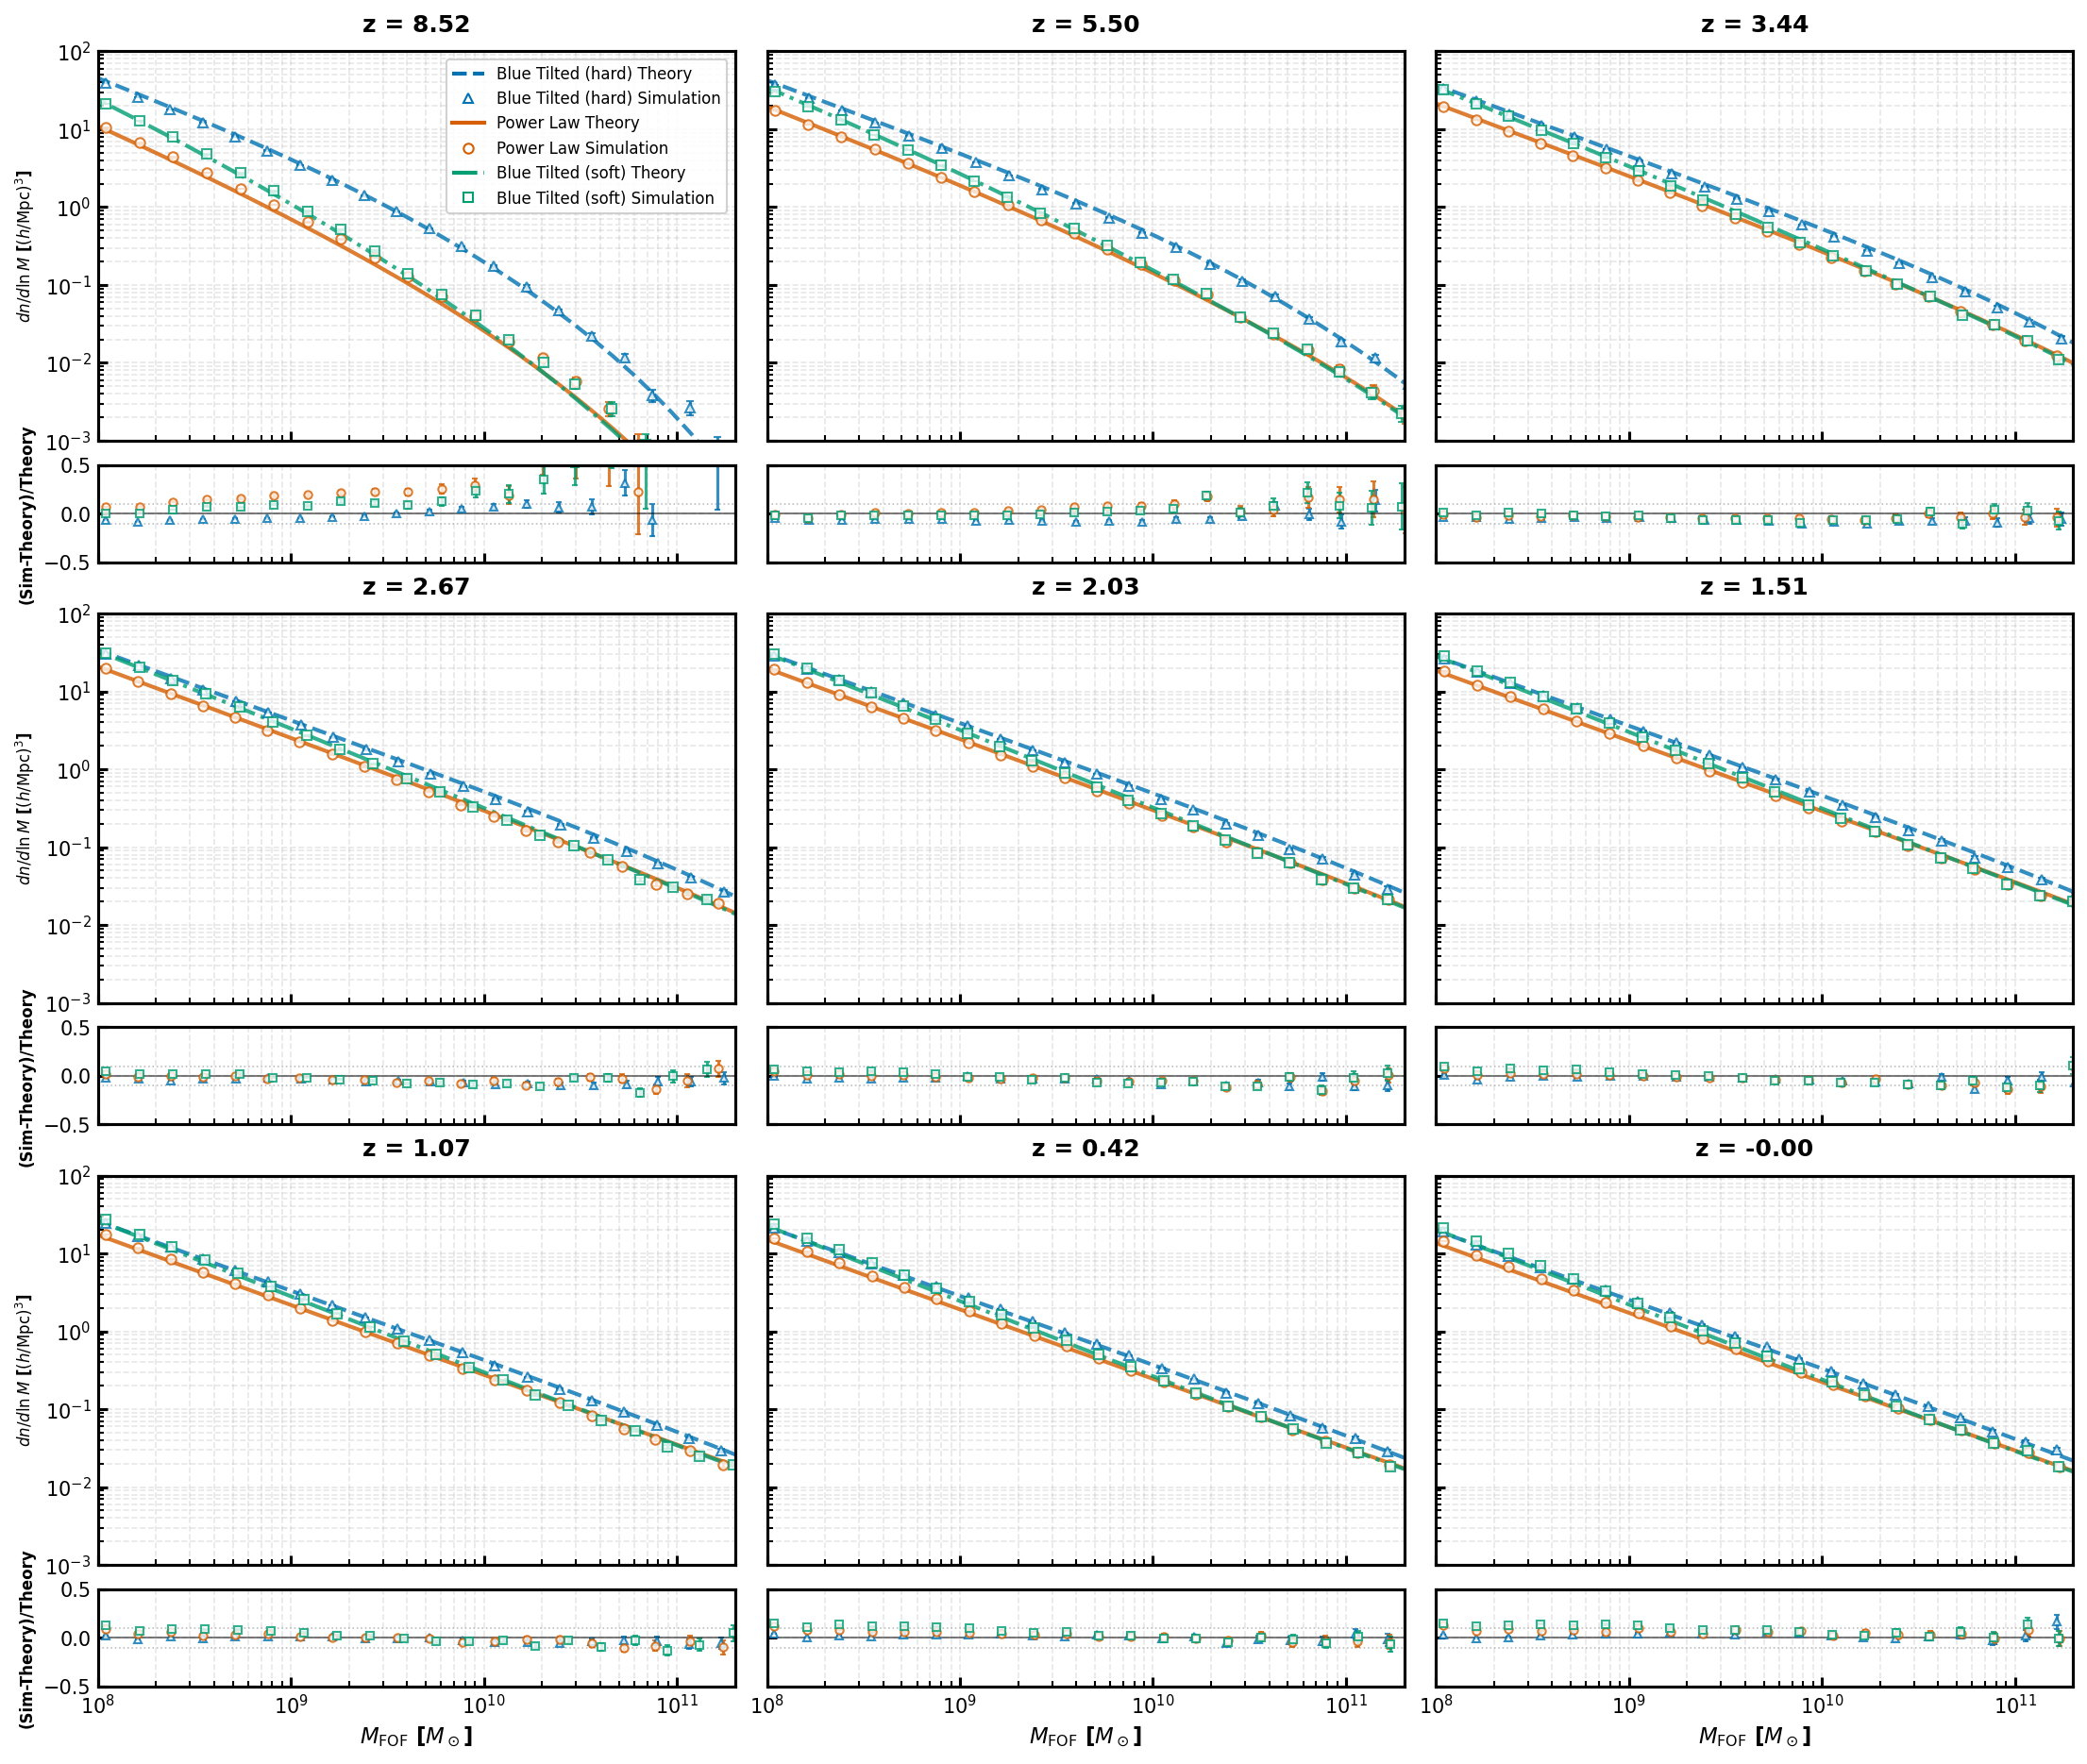
\includegraphics[scale=0.45]{mass_function_3models_comparison_3x3_grid_reed07_without_nu_Integral.png}
    \caption{Halo Mass Function Comparison Across Cosmological Models and Redshifts 2×2 panel showing the halo mass function dN/dlnM as a function of halo mass at different redshifts (z = 8.52, 3.44, 1.07, 0.00). Each panel compares simulation results from different cosmological models: CDM (Cold Dark Matter) shown only at z=0, and blue-tilted power spectrum models with kp=1 and kp=10 {\color{red} You need to say which 'deep' and 'soft' have kp and ms. }. Simulation data are represented by colored symbols with error bars, while theoretical predictions from Bocquet16 (200c) and Reed07 (FoF) mass function models are shown as gray lines. All simulations use 25 Mpc/h box size with 1024³ particles. Mass functions are computed using 200 times critical density definition and Poisson error estimates. The plots demonstrate how blue-tilted power spectra affect the abundance of dark matter halos across cosmic time, with the effect being more pronounced at higher redshifts. {\color{red} TK: Good. Excellent fit now!} {\color{red} In general, we should be more clear about the kp and ms in the plot. What is the kp and ms here?}}
    \label{fig:mass_function}
\end{figure*}

{\color{red} TK: we could write down explicitly the formula for analytic halo mass function here.}

\subsubsection{Half Mass Redshift\label{subsub:HMR}}
Figure X presents the redshift at which halos reach half of their final mass ($z_{1/2}$) as a function of their $z=0$ mass for three cosmological models: standard CDM (PL), the strongly blue-tilted model (BT, $k_p=1$), and the weakly blue-tilted model (BT, $k_p=10$). This quantity, also known as the half-mass epoch, serves as a fundamental indicator of halo assembly history, characterizing when the bulk of a halo's final mass was accreted. Our analysis is based on the mass evolution tracks of individual halos extracted from HBT+ halo merger trees across four initial mass bins spanning $10^{-3}$ to $10^{1}$ in units of $10^{10} M_{\odot}$.

The computation of $z_{1/2}$ follows a robust methodology: for each halo, we first determine its mass at $z=0$ ($M_{z=0}$). We then trace its mass evolution backward in time through 21 discrete redshift outputs (from $z=0$ to $z\approx8.5$), linearly interpolating between adjacent snapshots to identify the precise redshift when the halo's mass first drops below $M_{z=0}/2$. {\color{red} (the biggest progenitor or all progenitor mass?)} Halos that do not reach half of their final mass within the redshift range are excluded from the analysis {\color{red}, ensuring data reliability}.

To establish the mass dependence of the assembly history, halos are partitioned into distinct mass bins based on their $z=0$ mass in logarithmic space. The lowest mass bin ($10^{-3}$ to $10^{-2} \times 10^{10} M_{\odot}$) is treated as a single partition due to limited statistics, while each of the three higher mass bins is subdivided into five equally-spaced logarithmic sub-bins. For each resulting mass bin, we compute the mean and standard deviation of $z_{1/2}$ across all member halos.

The comparison reveals a clear mass-dependent assembly trend across all models: low-mass halos ($M_{z=0} \lesssim 10^{9} M_{\odot}$) assemble the majority of their mass earlier (higher $z_{1/2}$) compared to their high-mass counterparts ($M_{z=0} \gtrsim 10^{10} M_{\odot}$), consistent with hierarchical structure formation. However, the blue-tilted models exhibit systematic offsets relative to the standard CDM model. The strongly blue-tilted model (BT, $k_p=1$) shows the highest $z_{1/2}$ values across nearly all mass bins, indicating that halos in this model assemble their mass earlier. The weakly blue-tilted model (BT, $k_p=10$) generally falls between the other two models, though it approaches the standard CDM predictions at the highest masses. These differences are most pronounced at intermediate masses ($M_{z=0} \sim 10^{9} - 10^{10} M_{\odot}$), where the enhanced small-scale power in blue-tilted models promotes earlier halo formation and mass assembly.
This systematic shift in assembly history provides complementary evidence for the impact of blue-tilted primordial power spectra on structure formation, independent of halo abundance and density profile analyses. The earlier assembly of halos, particularly at intermediate masses, may have significant implications for the formation timescales of galaxies and the thermal history of the intergalactic medium in these models.

\subsubsection{concentration\label{subsub:concentration}}
{\color{blue}The concentration–mass relation is derived from halo catalogs generated by the \textsc{hbt+} halo finder applied to the outputs of the Blue-tilted and CDM simulations. we extract the halo mass \(M_{200c}\) and the corresponding concentration \(c_{200c}\) from the \texttt{SO/200\_crit} group of the HDF5 file. The masses are converted to solar masses by multiplying the stored values by the unit factor \(10^{10}\,M_{\odot}\). Only halos with positive masses are retained, and the mass is transformed to logarithmic scale, \(\log_{10}(M_{200c}/M_{\odot})\).

To characterize the median concentration as a function of mass, we bin the halos in logarithmic mass bins. The mass range from \(\log_{10}(M/M_{\odot}) = 8.0\) to \(13.5\) is divided into 100 equally spaced bins. Within each bin, we compute the median concentration as well as the 16th and 84th percentiles. The lower and upper error bars for the median are then defined as \(\mathrm{median} - P_{16}\) and \(P_{84} - \mathrm{median}\), respectively. These percentiles provide an estimate of the scatter in the concentration–mass relation.

Theoretical predictions for the concentration–mass relation are obtained using the \textsc{colossus} Python package \citep{Diemer2018}. We adopt two widely used models: the Diemer \& Joyce (2019) model \citep{Diemer2019} and the Ishiyama et al. (2021) model \citep{Ishiyama2021}. For each model, we compute the median concentration at the same redshifts as the simulation snapshots. The models require an input mass definition of \(M_{200c}\), which we adopt. Additionally, the power spectrum used in the model is specified via the \texttt{ps\_args} parameter. To match the two cosmological scenarios, we employ two different power spectra: the Eisenstein \& Hu (1998) transfer function \citep{Eisenstein1998} with the default power-law primordial spectrum (\texttt{eisenstein98\_pl}) for the CDM case, and a modified version with a blue-tilted primordial spectrum (\texttt{eisenstein98\_bt}) for the Blue-tilted simulation. The cosmological parameters are set consistently with the simulations: \(H_0 = 67.36\ \mathrm{km\,s^{-1}\,Mpc^{-1}}\), \(\Omega_m = 0.3153\), \(\Omega_b = 0.0493\), \(\sigma_8 = 0.8111\), and \(n_s = 0.9649\). The theoretical curves are then plotted over the same mass range as the binned simulation data, allowing a direct comparison between the simulated concentration–mass relations and the analytic predictions.

{\color{black}Figure~X presents a comparison of the halo concentration-mass relation across four key epochs, from high redshift ($z \approx 8.52$) to the present day ($z = 0.00$), for three distinct cosmological models: the standard Cold Dark Matter (CDM) model (PL), the strongly blue-tilted model (BT, $k_p=1$), and the weakly blue-tilted model (BT, $k_p=10$). The concentration is defined as $c_{200c} = R_{200c} / r_s$, where $R_{200c}$ is the spherical overdensity radius with respect to the critical density and $r_s$ is the scale radius of the NFW profile.

The analysis reveals a clear mass and redshift dependence in the concentration enhancement predicted by blue-tilted models. While all models exhibit the expected anti-correlation between concentration and halo mass, the divergence between the blue-tilted and standard models is most pronounced at low redshift. At $z=0$, the concentration of low-mass halos ($M_{200c} \sim 10^9 M_\odot$) in the strongly blue-tilted model ($k_p=1$) is a factor of 2 to 3 higher than in the standard CDM model. The weakly blue-tilted model ($k_p=10$) also shows significant enhancement, though to a lesser degree. This difference diminishes progressively with increasing redshift.

The redshift evolution of this effect follows a specific pattern: although the concentrations in blue-tilted models remain several times higher than in the standard model even at high redshift ($z \approx 8.52$), the relative magnitude of the divergence is greatest at $z=0$. This trend indicates that the distinct initial conditions set by the blue-tilted power spectrum are subsequently amplified through cosmic time. The nonlinear growth, merger history, and mass accretion processes that dominate structure formation at low redshifts act to solidify and magnify the differences in the internal structure of halos across the models. The ratio curves quantitatively confirm this evolution, showing the highest and steepest profiles (strongly mass-dependent) at $z=0$ and flatter, lower profiles at high redshift.

Theoretical predictions are in good overall agreement with the simulation trends, validating the implementation of the custom power spectra. Residual discrepancies at the high-redshift, low-mass end are likely attributable to simulation resolution limits or simplifications in the analytical concentration model under extreme conditions. The established evolutionary pattern---whereby concentration differences expand with cosmic time and peak at low redshift---provides a distinctive signature of blue-tilted primordial power spectra. It underscores that the impact of enhanced small-scale power is not only imprinted at halo formation but is also systematically leveraged by later nonlinear evolution. Consequently, observational constraints on the concentration of low-mass halos at low redshift will serve as a powerful probe for testing deviations from the standard scale-invariant primordial power spectrum.

{\color{red} TK: we could write down explicitly the formula for analytic theoretical prediction here. Explain why it works and the underlying assumption.}

\subsubsection{Power Spectrum\label{subsub:PS}}

\section{CONCLUSIONS}
\label{sec:conclusion}

\subsection{Halo Mass Function}
The blue-tilted models predict a significantly higher abundance of low-mass halos ($M < 10^{10} M_\odot$) at high redshifts ($z > 5$), indicating that enhanced small-scale power promotes the earlier collapse of low-mass structures. While the predictions of all models converge at the high-mass end towards lower redshifts, the abundance excess in blue-tilted models persists at the low-mass end, remaining a factor of 2--3 higher than the standard model at $z=0$.

\subsection{Dark Matter Power Spectrum}
A pronounced enhancement in small-scale power ($k > 1 \ h\mathrm{Mpc}^{-1}$) is present in the blue-tilted model across all redshifts. Crucially, this initial difference is dramatically amplified by non-linear evolution. By $z=0$, the non-linear matter power spectrum of the blue-tilted model exceeds that of the standard CDM model by over an order of magnitude at scales around $k \sim 10 \ h\mathrm{Mpc}^{-1}$.

\subsection{Half-Mass Epoch--Redshift Relation}
Halos of a given $z=0$ mass reach half of their final mass at a higher redshift in blue-tilted models compared to the standard model. This indicates an \textbf{earlier formation epoch} and a more rapid mass assembly history for halos in these models, with the effect being most pronounced for halos in the intermediate mass range ($10^9 \lesssim M_h \lesssim 10^{11} M_\odot$).

\subsection{Concentration-Mass Relation}
The blue-tilted models systematically produce halos with higher concentrations, with the effect being strongest at \textbf{low redshift} and for \textbf{low-mass halos}. At $z=0$, the concentration of low-mass halos can be 2--3 times higher than in the standard model. This enhancement weakens with increasing redshift, demonstrating that non-linear evolution acts to amplify the differences imprinted by the initial power spectrum.

\subsection{Halo Density Profile}
The density enhancement in blue-tilted models is primarily confined to the \textbf{inner regions} of halos ($r < 0.1 R_{200}$), while the outer density profiles remain similar to those in the standard model. This ``cuspy core'' structure suggests that the modified power spectrum predominantly affects the early collapse and central condensation of the halo.

\subsection{Synthesis: The Dark Matter Halo Population}
Collectively, these findings paint a coherent picture: a blue-tilted primordial power spectrum gives rise to a halo population that is \textbf{more abundant} at the low-mass end, forms \textbf{earlier}, and possesses \textbf{denser, more concentrated inner structures}. These effects point towards a universe where structure growth on small scales is accelerated and non-linear evolution is both advanced and intensified.

\section*{Acknowledgments}

\bibliographystyle{apsrev4-1-JHEPfix}
\bibliography{main}

\clearpage
\appendix

\end{document}
